% !TEX root = main.tex

\section*{Листочек 1: всего лишь функция} 
\addcontentsline{toc}{section}{Листочек 1: всего лишь функция}

\epigraph{Ты всего лишь машина, только имитация жизни. Робот сочинит симфонию? Робот превратит кусок холста в шедевр искусства?}{\textit{Из фильма <<Я, робот>> (2004)}}

%%%-------------------------------------------
\begin{problem}{(от регрессии к нейросетке)}
Однажды вечером, по пути с работы\footnote{она работает рисёрчером.} Маша зашла в свою любимую кофейню на Тверской. Там, на стене, она обнаружила очень интересную картину:

\begin{center}
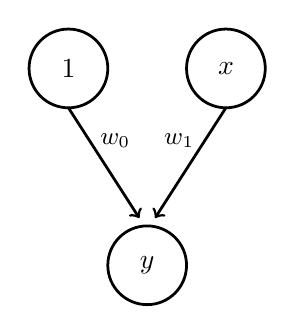
\begin{tikzpicture}[line cap=round,line join=round,x=1.0cm,y=1.0cm]

\draw [line width=1.pt] (0,1.5) circle (0.5cm) node {$1$};
\draw [line width=1.pt] (2,1.5) circle (0.5cm) node {$x$};
\draw [line width=1.pt] (1,-1) circle (0.5cm) node {$y$};

\draw [->, line width=1.pt] (0,1) -- (0.9,-0.4) node[pos=0.3,right] {\small $w_0$};
\draw [->, line width=1.pt] (2,1) -- (1.1,-0.4) node[pos=0.3,left] {\small $w_1$};
\end{tikzpicture}
\end{center}

Хозяин кофейни, Добродум, объяснил Маше, что это Покрас-Лампас так нарисовал линейную регрессию, и её легко можно переписать в виде формулы: $y_i = w_0 + w_1 \cdot x_i.$ Пока Добродум готовил кофе, Маша накидала у себя на бумажке новую картинку: 

\begin{center}
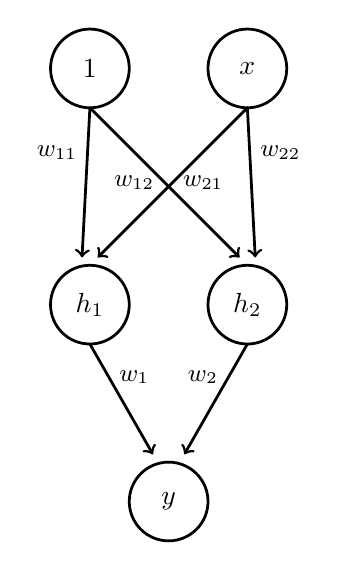
\begin{tikzpicture}[line cap=round,line join=round,x=1.0cm,y=1.0cm]

\draw [line width=1.pt] (0,2.5) circle (0.5cm) node {$1$};
\draw [line width=1.pt] (2,2.5) circle (0.5cm) node {$x$};

\draw [line width=1.pt] (0,-0.5) circle (0.5cm) node {$h_1$};
\draw [line width=1.pt] (2,-0.5) circle (0.5cm) node {$h_2$};

\draw [line width=1.pt] (1,-3) circle (0.5cm) node {$y$};

\draw [->, line width=1.pt] (0,2) -- (-0.1,0.1) node[pos=0.3,left] {\small $w_{11}$};
\draw [->, line width=1.pt] (2,2) -- (2.1,0.1) node[pos=0.3,right] {\small $w_{22}$};

\draw [->, line width=1.pt] (0,2) -- (1.9,0.1) node[pos=0.5,left] {\small $w_{12}$};
\draw [->, line width=1.pt] (2,2) -- (0.1,0.1) node[pos=0.5,right] {\small $w_{21}$};

\draw [->, line width=1.pt] (0,-1) -- (0.8,-2.4) node[pos=0.3,right] {\small $w_{1}$};
\draw [->, line width=1.pt] (2,-1) -- (1.2,-2.4) node[pos=0.3,left] {\small $w_{2}$};
\end{tikzpicture}
\end{center}

Как такая функция будет выглядеть в виде формулы? Правда ли, что $y$ будет нелинейно зависеть от $x$? Если нет, как это исправить и сделать зависимость нелинейной? 
\end{problem}

\newpage

\begin{sol}
Когда мы переписывали картинку в виде уравнения регрессии, мы брали вход из кругляшей, умножали его на веса, написанные около стрелок и искали сумму. Сделаем ровно то же самое для Машиной картинки. Величины $h_i$ внутри кругляшей скрытого слоя будут считаться как: 

\begin{equation*}
    \begin{aligned} 
    & h_1 = w_{11} \cdot 1 + w_{21} \cdot x \\
    & h_2 = w_{12} \cdot 1 + w_{22} \cdot x \\
    \end{aligned} 
\end{equation*}

Итоговый $y$ будет получаться из этих промежуточных величин как 

$$
y = w_1 \cdot h_1 + w_2 \cdot h_2.
$$

Подставим вместо $h_i$ их выражение через $x$ и получим уравнение, которое описывает картинку Маши

\begin{multline*} 
y = w_1 \cdot h_1 + w_2 \cdot h_2 = \\ = w_1 \cdot (w_{11} + w_{21} \cdot x)  + w_2 \cdot (w_{12} + w_{22} \cdot x)  = \\ = \underbrace{(w_1 w_{11} + w_2 w_{12})}_{\gamma_1} + \underbrace{(w_1 w_{21} + w_2 w_{22})}_{\gamma_2} \cdot x.
\end{multline*} 

Когда мы раскрыли скобки, мы получили ровно ту же самую линейную регрессию. Правда мы зачем-то довольно сложно параметризовали $\gamma_1$ и $\gamma_2$ через шесть параметров. Чтобы сделать зависимость нелинейной, нужно немного преобразить каждую из $h_i$, взяв от них какую-нибудь нелинейную функцию. Например, сигмоиду: 

$$
f(h) = \frac{1}{1 + e^{-h}}.
$$

Тогда формула преобразиться: 

$$
y = w_1 \cdot f(w_{11} + w_{21} \cdot x)  + w_2 \cdot f(w_{12} + w_{22} \cdot x).
$$

\sout{Смерти} Линейности больше нет. \indef{Только что на ваших глазах произошло чудо. Регрессия превратилась в нейросеть.} Можно использовать вместо сигмоиды любую другую функцию активации. Например, ReLU (Rectified Linear Unit) $$ReLU(h) = \max(0, h).$$
\end{sol} 

\newpage

%%%-------------------------------------------
\begin{problem}{(из картинки в формулу)}
Добродум хочет понять, насколько сильно будет заполнена кофейня в следующие выходные. Для этого он обучил нейросетку. На вход она принимает три фактора: температуру за окном, $x_1$, факт наличия на Тверской митинга, $x_2$ и пол баристы на смене, $x_3$.  В качестве функции активации Добродум использует $ReLU.$ 

\begin{center}
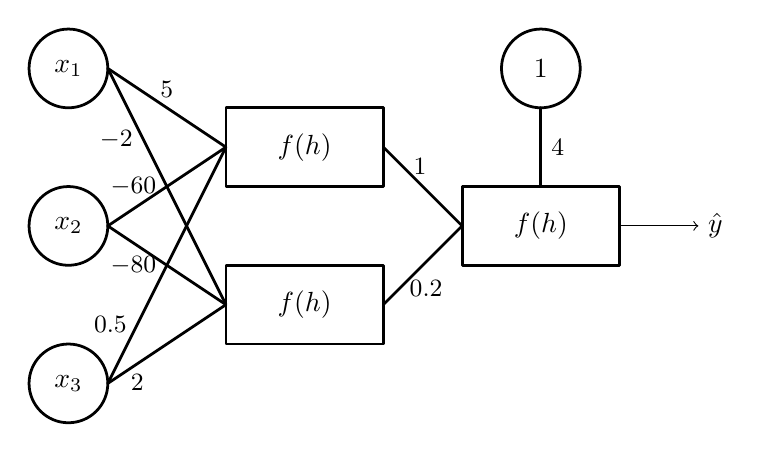
\begin{tikzpicture}[line cap=round,line join=round,x=1.0cm,y=1.0cm]

\draw [line width=1.pt] (-3,1.5) circle (0.5cm) node {$x_1$};
\draw [line width=1.pt] (-3,-0.5) circle (0.5cm) node {$x_2$};
\draw [line width=1.pt] (-3,-2.5) circle (0.5cm) node {$x_3$};	

\draw [line width=1.pt] (-1,0)--(1,0)--(1,1)--(-1,1)--cycle;
\draw (0,0.5) node {$f(h)$};
\draw [line width=1.pt] (-1,-2)--(1,-2)--(1,-1)--(-1,-1)--cycle;
\draw (0,-1.5) node {$f(h)$};

\draw [line width=1.pt] (3,1.5) circle (0.5cm) node {$1$};	
\draw [line width=1.pt] (2,-1)--(4,-1)--(4,0)--(2,0)--cycle;
\draw (3,-0.5) node {$f(h)$};

\draw [line width=1.pt] (-2.5,1.5) -- (-1,0.5) node[pos=0.5,above] {\small $5$};
\draw [line width=1.pt] (-2.5,1.5) -- (-1,-1.5) node[pos=0.3,left] {\small $-2$};
\draw [line width=1.pt] (-2.5,-0.5) -- (-1,0.5) node[pos=0.5,left] {\small $-60$};
\draw [line width=1.pt] (-2.5,-0.5) -- (-1,-1.5)  node[pos=0.5,left] {\small  $-80$};
\draw [line width=1.pt] (-2.5,-2.5) -- (-1,0.5) node[near start,left] {\small $0.5$};
\draw [line width=1.pt] (-2.5,-2.5) -- (-1,-1.5)  node[near start,below] {\small  $2$};

\draw [line width=1.pt] (1,0.5) -- (2,-0.5) node[pos=0.25,right] {\small $1$};
\draw [line width=1.pt] (1,-1.5) -- (2,-0.5) node[pos=0.2,right] {\small $0.2$};
\draw [line width=1.pt] (3,1) -- (3,0) node[pos=0.5,right] {\small  $4$};

\draw [->] (4,-0.5) -- (5,-0.5) node[right] {$\hat y$};
\end{tikzpicture}
\end{center}

\begin{enumerate}
\item В эти выходные за барной\footnote{барной... конечно, кофейня у него...} стойкой стоит Агнесса. Митинга не предвидится, температура будет в районе $20$ градусов. Спрогнозируйте, сколько человек придёт в кофейню к Добродуму? 

\item На самом деле каждая нейросетка --- это просто-напросто какая-то нелинейная сложная функция. Запишите нейросеть Добродума в виде функции.
\end{enumerate}
\end{problem}

\begin{sol}
Будем постепенно идти по сетке и делать вычисления. Подаём все значения в первый нейрон, получаем: 

$$
h_1 = \max(0, 5 \cdot 20 + (-60) \cdot 0 + 0.5 \cdot 1) = \max(0, 100.5) = 100.5
$$

Ровно то же самое делаем со вторым нейроном: 

$$
h_2 = \max(0, -2 \cdot 20 + (-80) \cdot 0 + 2 \cdot 1) = \max(0, -38) = 0
$$

Дальше результат скрытых нейронов идёт во второй слой: 

$$
\hat y = \max(0, 1 \cdot 100.5 + 0.2 \cdot 0 + 4 \cdot 1) = 104.5
$$

Это и есть итоговый прогноз.

\begin{center}
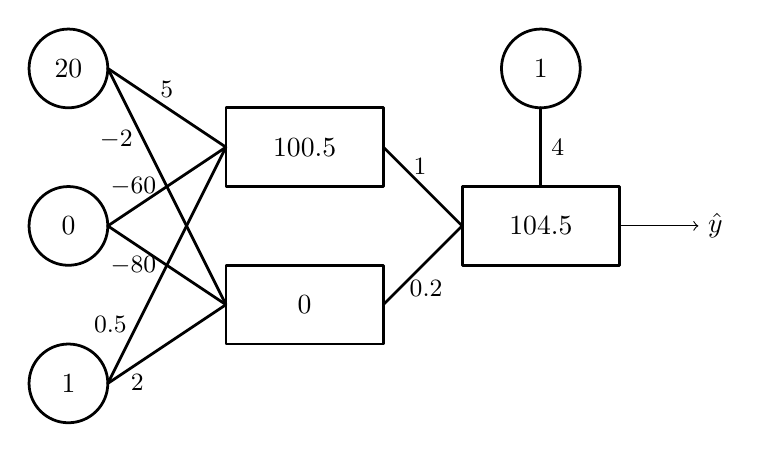
\begin{tikzpicture}[line cap=round,line join=round,x=1.0cm,y=1.0cm]

\draw [line width=1.pt] (-3,1.5) circle (0.5cm) node {$20$};
\draw [line width=1.pt] (-3,-0.5) circle (0.5cm) node {$0$};
\draw [line width=1.pt] (-3,-2.5) circle (0.5cm) node {$1$};	

\draw [line width=1.pt] (-1,0)--(1,0)--(1,1)--(-1,1)--cycle;
\draw (0,0.5) node {$100.5$};
\draw [line width=1.pt] (-1,-2)--(1,-2)--(1,-1)--(-1,-1)--cycle;
\draw (0,-1.5) node {$0$};

\draw [line width=1.pt] (3,1.5) circle (0.5cm) node {$1$};	
\draw [line width=1.pt] (2,-1)--(4,-1)--(4,0)--(2,0)--cycle;
\draw (3,-0.5) node {$104.5$};

\draw [line width=1.pt] (-2.5,1.5) -- (-1,0.5) node[pos=0.5,above] {\small $5$};
\draw [line width=1.pt] (-2.5,1.5) -- (-1,-1.5) node[pos=0.3,left] {\small $-2$};
\draw [line width=1.pt] (-2.5,-0.5) -- (-1,0.5) node[pos=0.5,left] {\small $-60$};
\draw [line width=1.pt] (-2.5,-0.5) -- (-1,-1.5)  node[pos=0.5,left] {\small  $-80$};
\draw [line width=1.pt] (-2.5,-2.5) -- (-1,0.5) node[near start,left] {\small $0.5$};
\draw [line width=1.pt] (-2.5,-2.5) -- (-1,-1.5)  node[near start,below] {\small  $2$};

\draw [line width=1.pt] (1,0.5) -- (2,-0.5) node[pos=0.25,right] {\small $1$};
\draw [line width=1.pt] (1,-1.5) -- (2,-0.5) node[pos=0.2,right] {\small $0.2$};
\draw [line width=1.pt] (3,1) -- (3,0) node[pos=0.5,right] {\small  $4$};

\draw [->] (4,-0.5) -- (5,-0.5) node[right] {$\hat y$};
\end{tikzpicture}
\end{center}

Теперь по мотивам наших вычислений запишем нейронку как функцию. Начинать будем с конца:

$$
\hat y = f(1 \cdot h_1 + 0.2 \cdot h_2 + 4 \cdot 1)
$$

Подставляем вместо $h_1$ и $h_2$ вычисления, которые происходят на первом слое нейронки: 

\begin{multline*}
\hat y = f(1 \cdot f(5 \cdot x_1 -60 \cdot x_2 + 0.5 \cdot x_3) + 0.2 \cdot f(-2 \cdot x_1 -80 \cdot x_2 + 2 \cdot x_3) + 4 \cdot 1) = \\ = \max(0, \max(0, 5 \cdot x_1 -60 \cdot x_2 + 0.5 \cdot x_3) + 0.2 \cdot \max(0, -2 \cdot x_1 -80 \cdot x_2 + 2 \cdot x_3) + 4).
\end{multline*}

Обучение нейронной сетки, на самом деле, эквивалентно обучению такой сложной нелинейной функции. 
\end{sol}

%\newpage 

%%%-------------------------------------------
\begin{problem}{(из формулы в картинку)}
Маша написала на бумажке функцию: 

\begin{equation*}
y = \max(0, 4 \cdot \max(0, 3 \cdot x_1 + 4 \cdot x_2 + 1) + 2 \cdot \max(0, 3 \cdot x_1 + 2 \cdot x_2 + 7) + 6)
\end{equation*} 

Теперь она хочет, чтобы кто-нибудь из её адептов нарисовал её в виде нейросетки. Нарисуйте.
\end{problem}

\begin{sol}
Начнём рисовать картинку с конца. На выход выплёвывается либо $0$, либо комбинация из двух входов: 

$$
\hat y = ReLU(4 \cdot h_1 + 2 \cdot h_2 + 6)
$$

Каждый из входов --- это снова либо $0$, либо комбинация из двух входов. 

$$
y = \max(0, {\color{red} 4} \cdot \underbrace{\max(0, 3 \cdot x_1 +  4 \cdot x_2 + 1)}_{h_1} + {\color{red} 2} \cdot \underbrace{\max(0, {\color{purp} 3} \cdot x_1 + {\color{purp} 2} \cdot x_2 + {\color{purp} 7})}_{h_2} + {\color{red} 6})
$$

Получается, что на первом слое находится два нейрона, которые передают свои выходы в третий:

\begin{center}
\begin{tikzpicture}[line cap=round,line join=round,x=1.0cm,y=1.0cm]

\draw [line width=1.pt] (-3,1.5) circle (0.5cm) node {$1$};
\draw [line width=1.pt] (-3,-0.5) circle (0.5cm) node {$x_1$};
\draw [line width=1.pt] (-3,-2.5) circle (0.5cm) node {$x_2$};	

\draw [line width=1.pt] (-1,0)--(1,0)--(1,1)--(-1,1)--cycle;
\draw (0,0.5) node {$ReLU$};
\draw (1,1) node[right] {$h_1$};
\draw [line width=1.pt] (-1,-2)--(1,-2)--(1,-1)--(-1,-1)--cycle;
\draw (0,-1.5) node {$ReLU$};
\draw (1,-2) node[right] {$h_2$};

\draw [line width=1.pt] (3,1.5) circle (0.5cm) node {$1$};	
\draw [line width=1.pt] (2,-1)--(4,-1)--(4,0)--(2,0)--cycle;
\draw (3,-0.5) node {$ReLU$};

\draw [line width=1.pt] (-2.5,1.5) -- (-1,0.5) node[near start,above] {\small $1$};
\draw [line width=1.pt, purp] (-2.5,1.5) -- (-1,-1.5) node[near start,right] {\small \color{purp} $7$};
\draw [line width=1.pt] (-2.5,-0.5) -- (-1,0.5) node[near start,above] {\small $3$};
\draw [line width=1.pt, purp] (-2.5,-0.5) -- (-1,-1.5)  node[near start,above] {\small \color{purp} $3$};
\draw [line width=1.pt] (-2.5,-2.5) -- (-1,0.5) node[near start,left] {\small $4$};
\draw [line width=1.pt, purp] (-2.5,-2.5) -- (-1,-1.5)  node[near start,below] {\small \color{purp} $2$};

\draw [line width=1.pt, red] (1,0.5) -- (2,-0.5) node[pos=0.5,above] {\small \color{red} $4$};
\draw [line width=1.pt, red] (1,-1.5) -- (2,-0.5) node[pos=0.5,below] {\small \color{red} $2$};
\draw [line width=1.pt, red] (3,1) -- (3,0) node[pos=0.5,right] {\small \color{red} $6$};

\draw [->] (4,-0.5) -- (5,-0.5) node[right] {$\hat y$};
\end{tikzpicture}
\end{center}
\end{sol}


%%%-------------------------------------------
\begin{problem}{(армия регрессий)}
Парни очень любят Машу,\footnote{когда у тебя есть лёрнинг, они так и лезут} а Маша с недавних пор любит собирать перcептроны и думать по вечерам об их весах и функциях активации. Сегодня она решила разобрать свои залежи из перcептронов и как следует упорядочить их. 

\begin{enumerate}
\item В ящике стола Маша нашла перcептрон с картинки \ref{perp1} Маша хочет подобрать веса так, чтобы он реализовывал логическое отрицание, то есть превращал $x_1 = 0$ в $y=1$, а $x_1 = 1$ в $y=0$. 

\begin{minipage}{0.49\linewidth}
\begin{figure}[H]
\caption{} \label{perp1}
\begin{center}
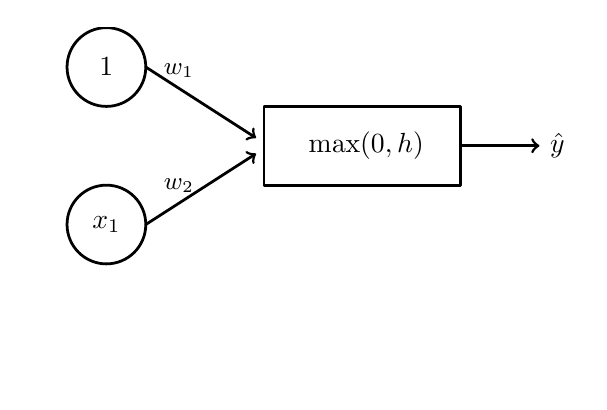
\begin{tikzpicture}[line cap=round,line join=round,x=1.0cm,y=1.0cm]
\clip(-4,0) rectangle (3,4.5); % чтобы выравнять картинки по размерам
\draw [line width=1.pt] (-3,4) circle (0.5cm) node {$1$};
\draw [line width=1.pt] (-3,2) circle (0.5cm) node {$x_1$};

\draw [line width=1.pt] (-1,3.5)--(-1,2.5)--(1.5,2.5)-- (1.5,3.5) -- cycle;

\draw [->, line width=1.pt] (-2.5,4) -- (-1.1,3.1) node[pos=0.3,above] {\small $w_1$};
\draw [->, line width=1.pt] (-2.5,2) -- (-1.1,2.9) node[pos=0.3,above] {\small $w_2$};
\draw [->, line width=1.pt] (1.5,3) -- (2.5,3) node[pos=1,right] {$\hat y$};
\draw (0.3,3) node {$\max(0,h)$};
\end{tikzpicture}
\end{center}
\end{figure}
\end{minipage}
\hfill
\begin{minipage}{0.49\linewidth}
\begin{figure}[H]
\caption{} \label{perp2}
\begin{center}
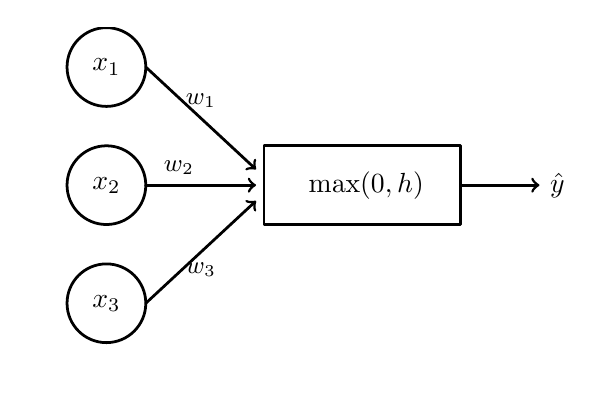
\begin{tikzpicture}[line cap=round,line join=round,x=1.0cm,y=1.0cm]
\clip(-4,0) rectangle (3,4.5);
\draw [line width=1.pt] (-3,4) circle (0.5cm) node {$x_1$};
\draw [line width=1.pt] (-3,2.5) circle (0.5cm) node {$x_2$};
\draw [line width=1.pt] (-3,1) circle (0.5cm) node {$x_3$};

\draw [line width=1.pt] (-1,3)--(-1,2)--(1.5,2)--(1.5,3)--cycle;
\draw (0.3,2.5) node {$\max(0,h)$};

\draw [->, line width=1.pt] (-2.5,4)--(-1.1,2.7) node[pos=0.5,above] {\small $w_1$};
\draw [->, line width=1.pt] (-2.5,2.5)--(-1.1,2.5) node[pos=0.3,above] {\small $w_2$};
\draw [->, line width=1.pt] (-2.5,1)--(-1.1,2.3) node[pos=0.5,below] {\small $w_3$};
\draw [->, line width=1.pt] (1.5,2.5)--(2.5,2.5) node[pos=1,right] {$\hat y$};
\end{tikzpicture}
\end{center}
\end{figure}
\end{minipage}

\item В тумбочке, среди носков, Маша нашла перcептрон, с картинки \ref{perp2}, Маша хочет подобрать такие веса $w_i$, чтобы персептрон превращал $x$ из таблички в соответствующие $y$:
	
\begin{center}
	\begin{tabular}{c|c|c|c}
    	$x_1$ & $x_2$ & $x_3$ & $y$ \\
    	\hline 
    	$1$ & $1$ & $2$ & $0.5$\\
    	\hline 
    	$1$ & $-1$ & $1$ & $0$ \\
	\end{tabular}
\end{center}

\item Оказывается, что в ванной всё это время валялась куча персептронов с картинки \ref{perp3} с неизвестной функцией активации.

\begin{minipage}{0.49\linewidth}
\begin{figure}[H]
\caption{} \label{perp3}
\begin{center}
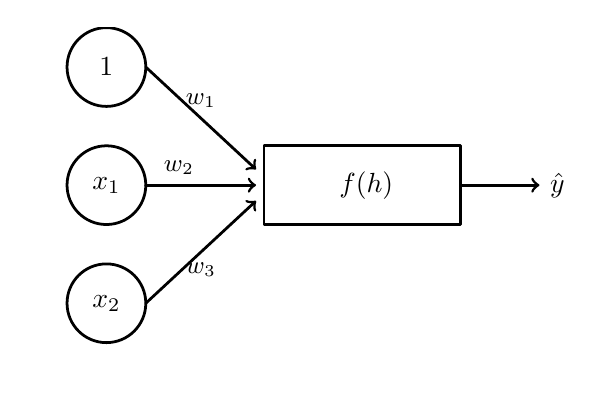
\begin{tikzpicture}[line cap=round,line join=round,x=1.0cm,y=1.0cm]
\clip(-4,0) rectangle (3,4.5);
\draw [line width=1.pt] (-3,4) circle (0.5cm) node {$1$};
\draw [line width=1.pt] (-3,2.5) circle (0.5cm) node {$x_1$};
\draw [line width=1.pt] (-3,1) circle (0.5cm) node {$x_2$};

\draw [line width=1.pt] (-1,3)--(-1,2)--(1.5,2)--(1.5,3)--cycle;
\draw (0.3,2.5) node {$f(h)$};

\draw [->, line width=1.pt] (-2.5,4)--(-1.1,2.7) node[pos=0.5,above] {\small $w_1$};
\draw [->, line width=1.pt] (-2.5,2.5)--(-1.1,2.5) node[pos=0.3,above] {\small $w_2$};
\draw [->, line width=1.pt] (-2.5,1)--(-1.1,2.3) node[pos=0.5,below] {\small $w_3$};
\draw [->, line width=1.pt] (1.5,2.5)--(2.5,2.5) node[pos=1,right] {$\hat y$};
\end{tikzpicture}
\end{center}
\end{figure}
\end{minipage}
\hfill
\begin{minipage}{0.49\linewidth}
\begin{figure}[H]
\caption{} \label{perp4}
\begin{center}
	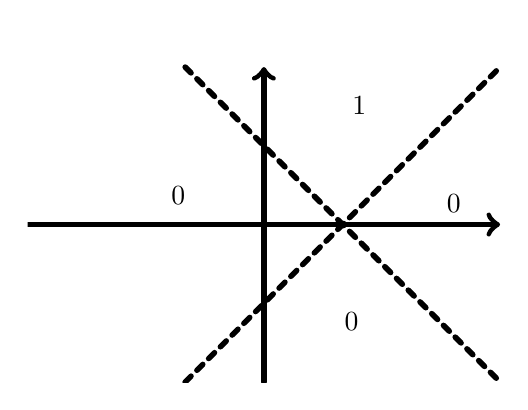
\begin{tikzpicture}[line cap=round,line join=round,x=1.0cm,y=1.0cm]
	\clip(-2,-5) rectangle (4,-0.5);
	\draw [->,line width=2.pt] (1,-5) -- (1,-1);
	\draw [->,line width=2.pt] (-2,-3) -- (4,-3);
	\draw (2,-1.25) node[anchor=north west] {$1$};
	\draw (-0.3,-2.4) node[anchor=north west] {$0$};
	\draw (1.9,-4) node[anchor=north west] {$0$};
	\draw (3.2,-2.5) node[anchor=north west] {$0$};	
	\draw [line width=2.pt,dash pattern=on 3pt off 3pt] (0,-5)-- (4,-1);
	\draw [line width=2.pt,dash pattern=on 3pt off 3pt] (0,-1)-- (4,-5);
	\end{tikzpicture}
\end{center}
\end{figure}
\end{minipage}

Маша провела на плоскости две прямые: $x_1 + x_2 = 1$ и $x_1 - x_2 = 1$. Она хочет собрать из персептронов нейросетку, которая будет классифицировать объекты с плоскости так, как показано на картинке \ref{perp4}. В качестве функции возьмите единичную ступеньку (Функцию Хевисайда). 
\end{enumerate}
\end{problem}

\begin{sol}
\vspace{-1.2cm} 
\begin{enumerate}
\item Начнём с первого пункта. Чтобы было легче запишем нейрон в виде уравнения: 

$$
\hat y = \max(0, w_1 + w_2 \cdot x_1).
$$

Нам нужно, чтобы 

\begin{equation*}
\begin{aligned}
\max(0, w_1 + w_2 \cdot 1) = 0 \\ 
\max(0, w_1 + w_2 \cdot 0) = 1 
\end{aligned}
\end{equation*}

На второе уравнение $w_2$ никак не влияет, а $w_1 = 1.$ Для того, чтобы в первом уравнении получить ноль, нужно взять любое $w_2 \le -1$. Нейрон готов. 

\item Снова выписываем несколько уравнений: 

\begin{equation*}
\begin{aligned}
\max(0, w_1 + w_2 + 2 \cdot w_3) = 0.5 \\ 
\max(0, w_1 - w_2 + w_3) = 0 
\end{aligned}
\end{equation*}

Тут решений может быть довольно много. Одно из них --- это занулить $w_1$ и $w_3$ в первом уравнении, а $w_2$ поставить $0.5$. Тогда во втором уравнении мы сразу же будем оказываться в отрицательной области и $ReLU$ заботливо будет отдавать нам $0$. 

\item Единичная ступенька выглядит как

$$
f(h) = \begin{cases} 1, h > 0 \\ 0, h \le 0 \end{cases}.
$$

Один нейрон --- это одна линия, проведённая на плоскости. Эта линия отделяет один класс от другого. Например, линию $ x_1 + x_2 - 1 = 0 $ мог бы описать нейрон 

\begin{minipage}{0.49\linewidth}
\begin{center}
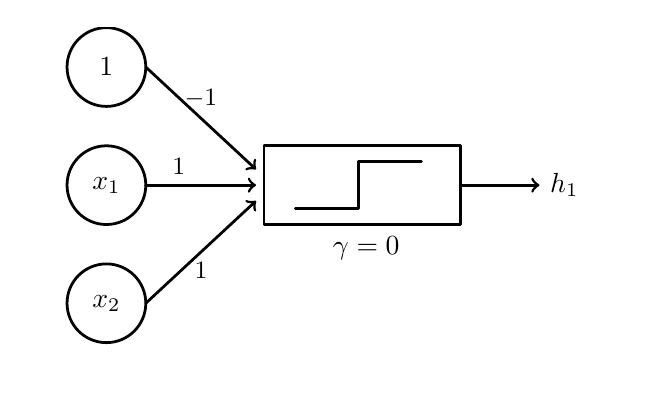
\begin{tikzpicture}[line cap=round,line join=round,x=1.0cm,y=1.0cm]
\clip(-4,0) rectangle (3.5,4.5);
\draw [line width=1.pt] (-3,4) circle (0.5cm) node {$1$};
\draw [line width=1.pt] (-3,2.5) circle (0.5cm) node {$x_1$};
\draw [line width=1.pt] (-3,1) circle (0.5cm) node {$x_2$};

\draw [line width=1.pt] (-1,3)--(-1,2)--(1.5,2)--(1.5,3)--cycle;
\draw [line width=1.pt] (-0.6,2.2)--(0.2,2.2)--(0.2,2.8)--(1,2.8);
\draw (0.3,1.7) node {$\gamma = 0$};

\draw [->, line width=1.pt] (-2.5,4)--(-1.1,2.7) node[pos=0.5,above] {\small $-1$};
\draw [->, line width=1.pt] (-2.5,2.5)--(-1.1,2.5) node[pos=0.3,above] {\small $1$};
\draw [->, line width=1.pt] (-2.5,1)--(-1.1,2.3) node[pos=0.5,below] {\small $1$};
\draw [->, line width=1.pt] (1.5,2.5)--(2.5,2.5) node[pos=1,right] {$h_1$};
\end{tikzpicture}
\end{center}
\end{minipage}
\hfill
\begin{minipage}{0.49\linewidth}
\begin{center}
	\begin{tikzpicture}[line cap=round,line join=round,x=1.0cm,y=1.0cm]
	\clip(0,-5) rectangle (4,-0.5);
 	\draw (2,-1.25) node[anchor=north west] {$1$};
 	\draw (0.3,-2.4) node[anchor=north west] {$0$};
	\draw [line width=2.pt,dash pattern=on 3pt off 3pt] (0,-1)-- (4,-5);
	\end{tikzpicture}
\end{center}
\end{minipage}

Порог $\gamma$ для кусочной функции в каком-то смысле дублирует константу. Они взаимосвязаны. Будем всегда брать его нулевым. Видим, что если мы получили комбинацию $x_1$, $x_2$ и $1$, большую, чем ноль, мы оказались справа от прямой. Если хочется поменять метки $0$ и $1$ местами, можно умножить все коэффициенты на $-1$. \indef{Наш персептрон понимает по какую сторону от прямой мы оказались,} то есть задаёт одну линейную разделяющую поверхность.  По аналогии для второй прямой мы можем получить следующий результат. 

\begin{minipage}{0.49\linewidth}
\begin{center}
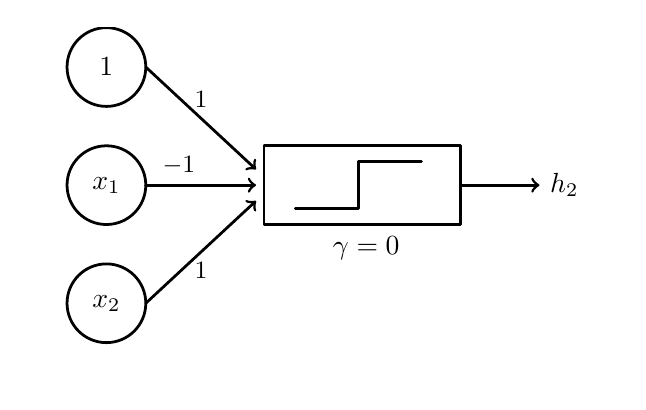
\begin{tikzpicture}[line cap=round,line join=round,x=1.0cm,y=1.0cm]
\clip(-4,0) rectangle (3.5,4.5);
\draw [line width=1.pt] (-3,4) circle (0.5cm) node {$1$};
\draw [line width=1.pt] (-3,2.5) circle (0.5cm) node {$x_1$};
\draw [line width=1.pt] (-3,1) circle (0.5cm) node {$x_2$};

\draw [line width=1.pt] (-1,3)--(-1,2)--(1.5,2)--(1.5,3)--cycle;
\draw [line width=1.pt] (-0.6,2.2)--(0.2,2.2)--(0.2,2.8)--(1,2.8);
\draw (0.3,1.7) node {$\gamma = 0$};

\draw [->, line width=1.pt] (-2.5,4)--(-1.1,2.7) node[pos=0.5,above] {\small $1$};
\draw [->, line width=1.pt] (-2.5,2.5)--(-1.1,2.5) node[pos=0.3,above] {\small $-1$};
\draw [->, line width=1.pt] (-2.5,1)--(-1.1,2.3) node[pos=0.5,below] {\small $1$};
\draw [->, line width=1.pt] (1.5,2.5)--(2.5,2.5) node[pos=1,right] {$h_2$};
\end{tikzpicture}
\end{center}
\end{minipage}
\hfill
\begin{minipage}{0.49\linewidth}
\begin{center}
	\begin{tikzpicture}[line cap=round,line join=round,x=1.0cm,y=1.0cm]
	\clip(0,-5) rectangle (4,-0.5);
 	\draw (2,-1.25) node[anchor=north west] {$1$};
 	\draw (1.9,-4) node[anchor=north west] {$0$};
 	\draw [line width=2.pt,dash pattern=on 3pt off 3pt] (0,-5)-- (4,-1);
	\end{tikzpicture}
\end{center}
\end{minipage}

Итак, первый персептрон выбрал нам позицию относительно первой прямой, второй относительно второй. Остаётся только объединить эти результаты. Нейрон для скрепки должен реализовать для нас логическую функцию, которую задаёт табличка ниже. Там же нарисованы примеры весов, которые могли бы объединить выхлоп первого слоя в итоговый прогноз.

\begin{minipage}{0.1\linewidth}
\begin{center}
\begin{tabular}{c|c|c}
	$h_1$ & $h_2$ & $\hat y$ \\
	\hline 
	$1$ & $1$ & {\color{green} $1$} \\
	\hline 
	$1$ & $0$ & {\color{green} $0$} \\
	\hline 
	$0$ & $1$ & {\color{green} $0$} \\
	\hline 
	$0$ & $0$ & {\color{green} $0$} \\
\end{tabular}
\end{center}
\end{minipage}
\hfill
\begin{minipage}{0.44\linewidth}
\begin{center}
	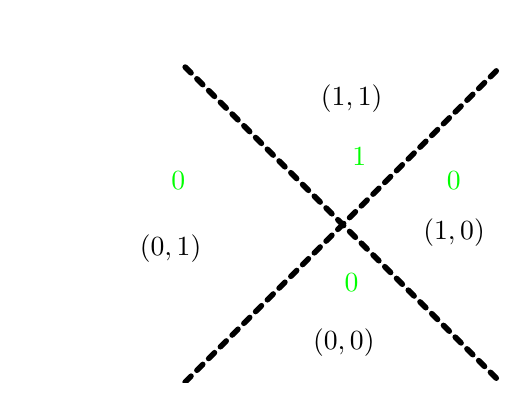
\begin{tikzpicture}[line cap=round,line join=round,x=1.0cm,y=1.0cm]
	\clip(-2,-5) rectangle (4,-0.5);
	
	\draw (2,-1.9) node[anchor=north west] {\color{green} $1$};
	\draw (1.6,-1.1) node[anchor=north west] {$(1, 1)$};
	
	\draw (-0.3,-2.2) node[anchor=north west] {\color{green} $0$};
	\draw (-0.7,-3) node[anchor=north west] {$(0, 1)$};
	
	\draw (1.9,-3.5) node[anchor=north west] {\color{green} $0$};
	\draw (1.5,-4.2) node[anchor=north west] {$(0, 0)$};
	
	\draw (3.2,-2.2) node[anchor=north west] {\color{green} $0$};	
	\draw (2.9,-2.8) node[anchor=north west] {$(1, 0)$};	
	
	\draw [line width=2.pt,dash pattern=on 3pt off 3pt] (0,-5)-- (4,-1);
	\draw [line width=2.pt,dash pattern=on 3pt off 3pt] (0,-1)-- (4,-5);
	\end{tikzpicture}
\end{center}
\end{minipage}
\hfill
\begin{minipage}{0.44\linewidth}
\begin{center}
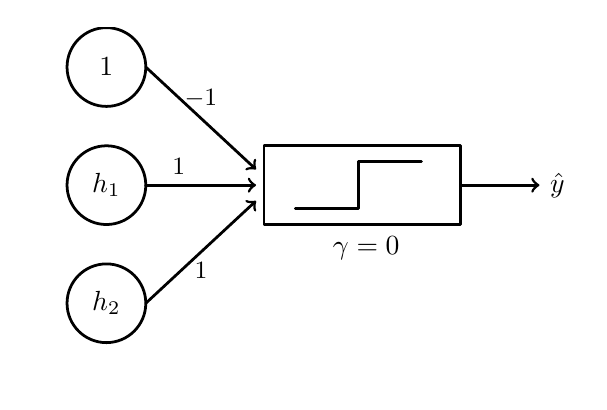
\begin{tikzpicture}[line cap=round,line join=round,x=1.0cm,y=1.0cm]
\clip(-4,0) rectangle (3,4.5);
\draw [line width=1.pt] (-3,4) circle (0.5cm) node {$1$};
\draw [line width=1.pt] (-3,2.5) circle (0.5cm) node {$h_1$};
\draw [line width=1.pt] (-3,1) circle (0.5cm) node {$h_2$};

\draw [line width=1.pt] (-1,3)--(-1,2)--(1.5,2)--(1.5,3)--cycle;
\draw [line width=1.pt] (-0.6,2.2)--(0.2,2.2)--(0.2,2.8)--(1,2.8);
\draw (0.3,1.7) node {$\gamma = 0$};

\draw [->, line width=1.pt] (-2.5,4)--(-1.1,2.7) node[pos=0.5,above] {\small $-1$};
\draw [->, line width=1.pt] (-2.5,2.5)--(-1.1,2.5) node[pos=0.3,above] {\small $1$};
\draw [->, line width=1.pt] (-2.5,1)--(-1.1,2.3) node[pos=0.5,below] {\small $1$};
\draw [->, line width=1.pt] (1.5,2.5)--(2.5,2.5) node[pos=1,right] {$\hat y$};
\end{tikzpicture}
\end{center}
\end{minipage}

Теперь мы можем нарисовать итоговую нейронную сеть, решающую задачу Маши. Она состоит из двух слоёв. Меньше не выйдет, так как каждый персептрон строит только одну разделяющую линию. 

\begin{center}
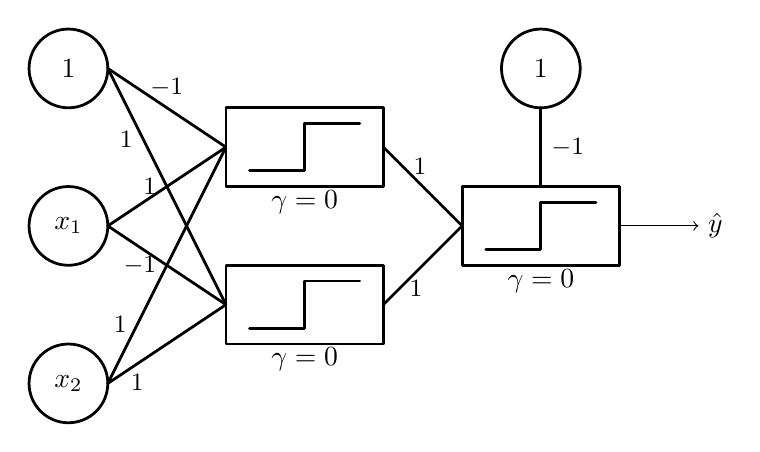
\begin{tikzpicture}[line cap=round,line join=round,x=1.0cm,y=1.0cm]

\draw [line width=1.pt] (-3,1.5) circle (0.5cm) node {$1$};
\draw [line width=1.pt] (-3,-0.5) circle (0.5cm) node {$x_1$};
\draw [line width=1.pt] (-3,-2.5) circle (0.5cm) node {$x_2$};	

\draw [line width=1.pt] (-1,0)--(1,0)--(1,1)--(-1,1)--cycle;
\draw [line width=1.pt] (-0.7,0.2)--(0,0.2)--(0,0.8)--(0.7,0.8);
\draw (0,-0.2) node {$\gamma = 0$};

\draw [line width=1.pt] (-1,-2)--(1,-2)--(1,-1)--(-1,-1)--cycle;
\draw [line width=1.pt] (-0.7,-1.8)--(0,-1.8)--(0,-1.2)--(0.7,-1.2);
\draw (0,-2.2) node {$\gamma = 0$};

\draw [line width=1.pt] (3,1.5) circle (0.5cm) node {$1$};	
\draw [line width=1.pt] (2,-1)--(4,-1)--(4,0)--(2,0)--cycle;
\draw [line width=1.pt] (2.3,-0.8)--(3,-0.8)--(3,-0.2)--(3.7,-0.2);
\draw (3,-1.2) node {$\gamma = 0$};

\draw [line width=1.pt] (-2.5,1.5) -- (-1,0.5) node[pos=0.5,above] {\small $-1$};
\draw [line width=1.pt] (-2.5,1.5) -- (-1,-1.5) node[pos=0.3,left] {\small $1$};
\draw [line width=1.pt] (-2.5,-0.5) -- (-1,0.5) node[pos=0.5,left] {\small $1$};
\draw [line width=1.pt] (-2.5,-0.5) -- (-1,-1.5)  node[pos=0.5,left] {\small  $-1$};
\draw [line width=1.pt] (-2.5,-2.5) -- (-1,0.5) node[near start,left] {\small $1$};
\draw [line width=1.pt] (-2.5,-2.5) -- (-1,-1.5)  node[near start,below] {\small  $1$};

\draw [line width=1.pt] (1,0.5) -- (2,-0.5) node[pos=0.25,right] {\small $1$};
\draw [line width=1.pt] (1,-1.5) -- (2,-0.5) node[pos=0.2,right] {\small $1$};
\draw [line width=1.pt] (3,1) -- (3,0) node[pos=0.5,right] {\small  $-1$};

\draw [->] (4,-0.5) -- (5,-0.5) node[right] {$\hat y$};
\end{tikzpicture}
\end{center}

Кстати говоря, если бы мы ввели для нашей нейросетки дополнительный признак $x_1 \cdot x_2$, у нас бы получилось обойтись только одним персептроном. В нашей ситуации \indef{нейросетка сама сварила на первом слое признак $x_1 \cdot x_2$, которого ей не хватало.} Другими словами говоря, нейросетка своим первым слоем превратила сложное пространство признаков в более простое, а затем вторым слоем, решила в нём задачу классификации. 
\end{enumerate}
\end{sol}


%%%-------------------------------------------
\begin{problem}{(логические функции)}
Маша вчера поссорилась с Пашей. Он сказал, что у неё нет логики. Чтобы доказать Паше обратное, Маша нашла теорему, которая говорит о том, что с помощью нейросетки можно аппроксимировать почти любую функцию, и теперь собирается заняться аппроксимацией логических функций. Для начала она взяла самые простые, заданные следующими таблицами истинности:

\begin{center}
\begin{minipage}{0.3\linewidth} 
\begin{tabular}{c|c|c}
	$x_1$ & $x_2$ & $x_1 \cap x_2$ \\
	\hline 
	$1$ & $1$ & $1$ \\
	\hline 
	$1$ & $0$ & $0$ \\
	\hline 
	$0$ & $1$ & $0$ \\
	\hline 
	$0$ & $0$ & $0$ \\
\end{tabular}
\end{minipage}
\hfill
\begin{minipage}{0.3\linewidth}
		\begin{tabular}{c|c|c}
		$x_1$ & $x_2$ & $x_1 \cup x_2$ \\
		\hline 
		$1$ & $1$ & $1$ \\
		\hline 
		$1$ & $0$ & $1$ \\
		\hline 
		$0$ & $1$ & $1$ \\
		\hline 
		$0$ & $0$ & $0$ \\
	\end{tabular}
\end{minipage}
\hfill
\begin{minipage}{0.3\linewidth}
		\begin{tabular}{c|c|c}
		$x_1$ & $x_2$ & $x_1 \mbox{ } XoR \mbox{ } x_2$ \\
		\hline 
		$1$ & $1$ & $0$ \\
		\hline 
		$1$ & $0$ & $1$ \\
		\hline 
		$0$ & $1$ & $1$ \\
		\hline 
		$0$ & $0$ & $0$ \\
	\end{tabular}
\end{minipage}
\end{center}

Первые два столбика идут на вход, третий получается на выходе. Первая операция --- логическое "и", вторая --- "или".   Операция из третьей таблицы называется "исключающим или", $(XoR)$. Если внимательно приглядеться, то можно заметить, что $XoR$ --- это то же самое что и $[x_1 \ne x_2]$\footnote{Тут квадратные скобки обозначают индикатор. Он выдаёт $1$, если внутри него стоит правда и $0$, если ложь. Такая запись называется скобкой Айверсона. Попробуйте записать через неё единичную ступеньку Хевисайда.}. 
\end{problem}

\begin{sol} 
На самом деле, в предыдущем упражнении, мы уже построили нейрон для пересечения. Он располагался на последнем слое нейросети. Посмотрим на тот же нейрон под другим углом:

\begin{minipage}{0.29\linewidth}
\begin{center}
	\begin{tikzpicture}[line cap=round,line join=round,x=1.0cm,y=1.0cm]
    
    \draw [->, line width=1.pt] (-0.3,0) --(3.5,0); 
    \draw [->, line width=1.pt] (0,-0.3) --(0,3.5); 
    
    \draw [fill=blue] (0,0) circle (4pt);
    \draw [fill=blue] (0,2) circle (4pt);
    \draw [fill=blue] (2,0) circle (4pt);
    \path (2,2) pic[red] {cross=4pt};
    \draw [line width=2.pt,dash pattern=on 3pt off 3pt] (-0.4,3.2)-- (3.2,-0.4);
	\end{tikzpicture}
\end{center}
\end{minipage}
\hfill
\begin{minipage}{0.59\linewidth}
\begin{center}
\begin{tikzpicture}[line cap=round,line join=round,x=1.0cm,y=1.0cm]
\clip(-4,0) rectangle (3,4.5);
\draw [line width=1.pt] (-3,4) circle (0.5cm) node {$1$};
\draw [line width=1.pt] (-3,2.5) circle (0.5cm) node {$x_1$};
\draw [line width=1.pt] (-3,1) circle (0.5cm) node {$x_2$};

\draw [line width=1.pt] (-1,3)--(-1,2)--(1.5,2)--(1.5,3)--cycle;
\draw [line width=1.pt] (-0.6,2.2)--(0.2,2.2)--(0.2,2.8)--(1,2.8);
\draw (0.3,1.7) node {$\gamma = 0$};

\draw [->, line width=1.pt] (-2.5,4)--(-1.1,2.7) node[pos=0.5,above] {\small $-\tfrac{3}{2}$};
\draw [->, line width=1.pt] (-2.5,2.5)--(-1.1,2.5) node[pos=0.3,above] {\small $1$};
\draw [->, line width=1.pt] (-2.5,1)--(-1.1,2.3) node[pos=0.5,below] {\small $1$};
\draw [->, line width=1.pt] (1.5,2.5)--(2.5,2.5) node[pos=1,right] {$\hat y$};
\end{tikzpicture}
\end{center}
\end{minipage}

Если нарисовать все наши четыре точки на плоскости, становится ясно, что мы хотим отделить точку $(1,1)$ от всех остальных. Сделать это можно большим числом способов. Например, в нейроне выше задана линия $x_2 = 1.5 - x_1$. Подойдёт и любая другая линия, отделяющая $(1,1)$ от остальных точек. Пропустим ради приличия точки через наш нейрон и убедимся, что он работает корректно:

\begin{equation*}
\begin{aligned}
& [-1.5 + 1 + 1 > 0] = [0.5 > 0] = 1 \\
& [-1.5 + 0 + 0 > 0] = [-1.5 > 0] = 0 \\
& [-1.5 + 0 + 1 > 0] = [-0.5 > 0] = 0 \\
& [-1.5 + 1 + 0 > 0] = [-0.5 > 0] = 0 \\
\end{aligned}
\end{equation*}

С объединением та же ситуация, только на этот раз линия должна пройти чуть ниже. Подойдёт $x_2 = 0.5 - x_1$.

\begin{minipage}{0.29\linewidth}
\begin{center}
	\begin{tikzpicture}[line cap=round,line join=round,x=1.0cm,y=1.0cm]
    
    \draw [->, line width=1.pt] (-0.3,0) --(3.5,0); 
    \draw [->, line width=1.pt] (0,-0.3) --(0,3.5); 
    
    \draw [fill=blue] (0,0) circle (4pt);
    \path (0,2) pic[red] {cross=4pt};
    \path (2,0) pic[red] {cross=4pt};
    \path (2,2) pic[red] {cross=4pt};
    \draw [line width=2.pt,dash pattern=on 3pt off 3pt] (-0.4,1.6)-- (1.6,-0.4);
	\end{tikzpicture}
\end{center}
\end{minipage}
\hfill
\begin{minipage}{0.59\linewidth}
\begin{center}
\begin{tikzpicture}[line cap=round,line join=round,x=1.0cm,y=1.0cm]
\clip(-4,0) rectangle (3,4.5);
\draw [line width=1.pt] (-3,4) circle (0.5cm) node {$1$};
\draw [line width=1.pt] (-3,2.5) circle (0.5cm) node {$x_1$};
\draw [line width=1.pt] (-3,1) circle (0.5cm) node {$x_2$};

\draw [line width=1.pt] (-1,3)--(-1,2)--(1.5,2)--(1.5,3)--cycle;
\draw [line width=1.pt] (-0.6,2.2)--(0.2,2.2)--(0.2,2.8)--(1,2.8);
\draw (0.3,1.7) node {$\gamma = 0$};

\draw [->, line width=1.pt] (-2.5,4)--(-1.1,2.7) node[pos=0.5,above] {\small $-\tfrac{1}{2}$};
\draw [->, line width=1.pt] (-2.5,2.5)--(-1.1,2.5) node[pos=0.3,above] {\small $1$};
\draw [->, line width=1.pt] (-2.5,1)--(-1.1,2.3) node[pos=0.5,below] {\small $1$};
\draw [->, line width=1.pt] (1.5,2.5)--(2.5,2.5) node[pos=1,right] {$\hat y$};
\end{tikzpicture}
\end{center}
\end{minipage}

С третьей операцией, исключающим или, начинаются проблемы. Чтобы разделить точки, нужно строить две линии. Сделать это можно многими способами. Но линий всегда будет две. То есть мы попадаем в ситуацию из прошлой задачки. Надо посмотреть первым слоем нейросетки, где мы оказались относительно каждой из линий, а вторым слоем соединить результаты. 

\begin{minipage}{0.45\linewidth}
\begin{center}
	\begin{tikzpicture}[line cap=round,line join=round,x=1.0cm,y=1.0cm]
    
    \draw [->, line width=1.pt] (-0.3,0) --(3.5,0); 
    \draw [->, line width=1.pt] (0,-0.3) --(0,3.5); 
    
    \draw [fill=blue] (0,0) circle (4pt);
    \path (0,2) pic[red] {cross=4pt};
    \path (2,0) pic[red] {cross=4pt};
    \draw [fill=blue] (2,2) circle (4pt);
    \draw [line width=2.pt,dash pattern=on 3pt off 3pt] (-0.4,1.6)-- (1.6,-0.4);
    \draw [line width=1.pt] (-0.4,3.2)-- (3.2,-0.4);
	\end{tikzpicture}
\end{center}
\end{minipage}
\hfill 
\begin{minipage}{0.45\linewidth}
\begin{center}
	\begin{tikzpicture}[line cap=round,line join=round,x=1.0cm,y=1.0cm]
    
    \draw [->, line width=1.pt] (-0.3,0) --(3.5,0); 
    \draw [->, line width=1.pt] (0,-0.3) --(0,3.5); 
    
    \draw [fill=blue] (0,0) circle (4pt);
    \path (0,2) pic[red] {cross=4pt};
    \path (2,0) pic[red] {cross=4pt};
    \draw [fill=blue] (2,2) circle (4pt);
    \draw [line width=2.pt,dash pattern=on 3pt off 3pt] (-0.3,1)-- (2.7,1);
    \draw [line width=1.pt] (1,-0.3)-- (1,2.7);
	\end{tikzpicture}
\end{center}
\end{minipage}

Если немного пофантазировать, можно даже записать эту нейросеть через объединение и пересечение: 

$$
\hat y = [1 \cdot (x_1 \cup x_2) - 1 \cdot (x_1 \cap x_2) - 0.5 > 0]
$$

Нейрон $(x_1 \cup x_2)$ выясняет по какую сторону от сплошной линии мы оказались, нейрон $x_1 \cap x_2$ делает то же самое для пунктирной линии. А дальше мы просто объединяем результат.
\end{sol}

%%%-------------------------------------------
\begin{problem}{(ещё немного про XoR)} 
Маша заметила, что на $XoR$ ушло очень много персептронов. Она поняла, что первые два персептрона пытаются сварить для третьего нелинейные признаки, которых нейросетке не хватает. Она решила самостоятельно добавить персептрону вход $x_3 = x_1 \cdot x_2$ и реализовать XoR одним персептроном. Можно ли это сделать? 
\end{problem}

\begin{sol}
Маша обратила внимание на очень важную штуку. Нам не хватает признаков, чтобы реализовать $XoR$ за один нейрон. Поэтому первый слой нейросетки сам их для нас придумывает. Чем глубже нейросетку мы построим, тем более сложные и абстрактные признаки она будет выделять из данных. Если добавить ко входу $x_3 = x_1 \cdot x_2$, мы сделаем за нейросетку часть её работы и сможем обойтись одним нейроном. Например, вот таким: 

$$
\hat y = [x_1 + x_2 - 2\cdot x_1 \cdot x_2 - 0.5 > 0]
$$

Такая линия как раз будет задавать две скрещивающиеся прямые. 

\begin{center}
	\begin{tikzpicture}[line cap=round,line join=round,x=1.0cm,y=1.0cm]
    
    \draw [->, line width=1.pt] (-0.3,0) --(3.5,0); 
    \draw [->, line width=1.pt] (0,-0.3) --(0,3.5); 
    
    \draw [fill=blue] (0,0) circle (4pt);
    \path (0,2) pic[red] {cross=4pt};
    \path (2,0) pic[red] {cross=4pt};
    \draw [fill=blue] (2,2) circle (4pt);
    \draw [line width=2.pt,dash pattern=on 3pt off 3pt] (-0.3,1)-- (2.7,1);
    \draw [line width=1.pt] (1,-0.3)-- (1,2.7);
	\end{tikzpicture}
\end{center}

Это легко увидеть, если немного поколдовать над уравнением: 

\begin{equation*}
\begin{aligned}
& x_1 + x_2 - 2x_1x_2 - 0.5 = 0 \\
& 2x_1 + 2x_2 - 4x_1 x_2 - 1 = 0 \\ 
& 2x_1(1 - 2 x_2) + 2 x_2 - 1 = 0 \\
& (1 - 2 x_2) \cdot (2 x_1 - 1) = 0
\end{aligned}
\end{equation*}

Получаем два решения. Прямую $x_2 = 0.5$ и прямую $x_1 = 0.5$.
\end{sol} 

% \newpage
% %%%-------------------------------------------
% \begin{problem}{(универсальный классификатор)}
% Маша задумалась о том, можно ли с помощью нейронной сетки решить абсолютно любую задачу классификации на два класса со сколь угодно большой точностью. Как думаете будет ли достаточно одного скрытого слоя и ступенчатой функции активации?
% \end{problem} 

% \begin{sol}
% Сейчас мы покажем, что нейросеть может решить любую задачу классификации с любой точностью\footnote{Не нужно воспринимать это, как формальное доказательство, это всего лишь "Показательство".}. Для начала попробуем решить задачку с картинки ниже одним нейроном:

% \begin{center}
% \begin{tikzpicture}[scale = 0.7, line cap=round,line join=round,x=1.0cm,y=1.0cm]
% \draw [fill=blue] (-1.66,5.46) circle (2.5pt);
% \draw [fill=blue] (-2.1,4.78) circle (2.5pt);
% \draw [fill=blue] (-1.64,3.84) circle (2.5pt);
% \draw [fill=blue] (-0.2,3.38) circle (2.5pt);
% \draw [fill=blue] (1.42,3.) circle (2.5pt);
% \draw [fill=blue] (1.98,2.58) circle (2.5pt);
% \draw [fill=blue] (1.76,1.62) circle (2.5pt);
% \draw [fill=blue] (1.56,1.32) circle (2.5pt);
% \draw [fill=blue] (1.,1.02) circle (2.5pt);
% \draw [fill=blue] (0.24,0.52) circle (2.5pt);
% \draw [fill=blue] (0.06,-0.28) circle (2.5pt);
% \draw [fill=blue] (-0.16,1.7) circle (2.5pt);
% \draw [fill=blue] (0.8,1.68) circle (2.5pt);
% \draw [fill=blue] (0.78,2.94) circle (2.5pt);
% \draw [fill=blue] (-0.7,2.58) circle (2.5pt);
% \draw [fill=blue] (-2.28,2.46) circle (2.5pt);
% \draw [fill=blue] (-2.32,3.56) circle (2.5pt);
% \draw [fill=blue] (-2.84,4.34) circle (2.5pt);
% \draw [fill=blue] (-2.78,5.22) circle (2.5pt);
% \draw [fill=blue] (-3.18,2.82) circle (2.5pt);
% \draw [fill=blue] (-1.44,3.12) circle (2.5pt);
% \draw [fill=blue] (-1.62,1.) circle (2.5pt);
% \draw [fill=blue] (-2.7,1.54) circle (2.5pt);
% \draw [fill=blue] (-1.36,1.88) circle (2.5pt);
% \draw [fill=blue] (-0.58,1.32) circle (2.5pt);
% \draw [fill=blue] (-0.9,-1.28) circle (2.5pt);
% \draw [fill=blue] (-0.94,0.68) circle (2.5pt);
% \draw [fill=blue] (1.48,-1.32) circle (2.5pt);
% \draw [fill=blue] (0.52,-1.24) circle (2.5pt);
% \draw [fill=blue] (-1.04,-0.34) circle (2.5pt);
% \draw [fill=blue] (0.42,-1.86) circle (2.5pt);
% \draw [fill=blue] (-2.02,0.16) circle (2.5pt);
% \draw [fill=blue] (-2.16,1.56) circle (2.5pt);
% \draw [fill=blue] (-3.26,3.46) circle (2.5pt);
% \draw [fill=blue] (-3.78,4.32) circle (2.5pt);
% \draw [fill=blue] (-3.52,4.82) circle (2.5pt);
% \draw [fill=blue] (-2.38,5.82) circle (2.5pt);
% \draw [fill=blue] (-1.28,5.98) circle (2.5pt);
% \draw [fill=blue] (1.72,-1.98) circle (2.5pt);
% \draw [fill=blue] (3.08,-2.06) circle (2.5pt);
% \draw [fill=blue] (2.1,-1.52) circle (2.5pt);
% \draw [fill=blue] (2.8,-1.36) circle (2.5pt);
% \path (0.44,5.76) pic[red] {cross=2.5pt};
% \path (-0.48,5.56) pic[red] {cross=2.5pt};
% \path (-0.68,5.) pic[red] {cross=2.5pt};
% \path (-0.64,4.12) pic[red] {cross=2.5pt};
% \path (-1.32,4.68) pic[red] {cross=2.5pt};
% \path (0.2,4.28) pic[red] {cross=2.5pt};
% \path (0.1,5.06) pic[red] {cross=2.5pt};
% \path (1.88,5.04) pic[red] {cross=2.5pt};
% \path (-1.28,5.38) pic[red] {cross=2.5pt};
% \path (1.,3.92) pic[red] {cross=2.5pt};
% \path (0.88,5.28) pic[red] {cross=2.5pt};
% \path (-0.82,3.42) pic[red] {cross=2.5pt};
% \path (0.22,2.7) pic[red] {cross=2.5pt};
% \path (1.22,2.42) pic[red] {cross=2.5pt};
% \path (1.78,3.32) pic[red] {cross=2.5pt};
% \path (2.76,2.24) pic[red] {cross=2.5pt};
% \path (2.2,0.44) pic[red] {cross=2.5pt};
% \path (1.54,0.6) pic[red] {cross=2.5pt};
% \path (0.94,0.34) pic[red] {cross=2.5pt};
% \path (0.88,-0.12) pic[red] {cross=2.5pt};
% \path (1.12,-0.62) pic[red] {cross=2.5pt};
% \path (2.06,-0.62) pic[red] {cross=2.5pt};
% \path (1.62,0.06) pic[red] {cross=2.5pt};
% \path (2.28,1.04) pic[red] {cross=2.5pt};
% \path (2.24,1.84) pic[red] {cross=2.5pt};
% \path (3.98,2.26) pic[red] {cross=2.5pt};
% \path (3.02,3.12) pic[red] {cross=2.5pt};
% \path (0.12,3.42) pic[red] {cross=2.5pt};
% \path (0.56,3.5) pic[red] {cross=2.5pt};
% \path (2.04,4.24) pic[red] {cross=2.5pt};
% \path (0.98,4.68) pic[red] {cross=2.5pt};
% \path (2.66,3.78) pic[red] {cross=2.5pt};
% \path (3.36,1.42) pic[red] {cross=2.5pt};
% \path (2.94,0.44) pic[red] {cross=2.5pt};
% \path (2.94,-0.44) pic[red] {cross=2.5pt};
% \path (3.78,-1.12) pic[red] {cross=2.5pt};
% \path (3.74,-1.86) pic[red] {cross=2.5pt};
% \path (3.34,-0.84) pic[red] {cross=2.5pt};
% \path (4.,0.32) pic[red] {cross=2.5pt};
% \path (3.92,0.96) pic[red] {cross=2.5pt};
% \path (3.6,1.88) pic[red] {cross=2.5pt};
% \path (3.54,2.66) pic[red] {cross=2.5pt};
% \path (2.38,2.92) pic[red] {cross=2.5pt};
% \path (4.04,-0.46) pic[red] {cross=2.5pt};
% \path (4.64,-1.66) pic[red] {cross=2.5pt};
% \path (4.36,-0.98) pic[red] {cross=2.5pt};
% \path (1.44,5.66) pic[red] {cross=2.5pt};
% \path (1.2,1.74) pic[red] {cross=2.5pt};
% \draw [line width=2.pt,dash pattern=on 3pt off 3pt] (0,-3)-- (0,7);
% \end{tikzpicture}
% \end{center} 

% Такая разделяющая полоса будет давать нам какое-то число ошибок. Как улучшить результат работы такой нейронки? Ответ прост: Давайте возьмём на первом слое два нейрона. Каждый из них построит по линии. На втором слое возьмём один нейрон, который объединит результат работы первого слоя и скажет нам, где именно мы оказались. Тогда получим такое решение: 

% \begin{center}
% \begin{tikzpicture}[scale = 0.7, line cap=round,line join=round,x=1.0cm,y=1.0cm]
% \draw [fill=blue] (-1.66,5.46) circle (2.5pt);
% \draw [fill=blue] (-2.1,4.78) circle (2.5pt);
% \draw [fill=blue] (-1.64,3.84) circle (2.5pt);
% \draw [fill=blue] (-0.2,3.38) circle (2.5pt);
% \draw [fill=blue] (1.42,3.) circle (2.5pt);
% \draw [fill=blue] (1.98,2.58) circle (2.5pt);
% \draw [fill=blue] (1.76,1.62) circle (2.5pt);
% \draw [fill=blue] (1.56,1.32) circle (2.5pt);
% \draw [fill=blue] (1.,1.02) circle (2.5pt);
% \draw [fill=blue] (0.24,0.52) circle (2.5pt);
% \draw [fill=blue] (0.06,-0.28) circle (2.5pt);
% \draw [fill=blue] (-0.16,1.7) circle (2.5pt);
% \draw [fill=blue] (0.8,1.68) circle (2.5pt);
% \draw [fill=blue] (0.78,2.94) circle (2.5pt);
% \draw [fill=blue] (-0.7,2.58) circle (2.5pt);
% \draw [fill=blue] (-2.28,2.46) circle (2.5pt);
% \draw [fill=blue] (-2.32,3.56) circle (2.5pt);
% \draw [fill=blue] (-2.84,4.34) circle (2.5pt);
% \draw [fill=blue] (-2.78,5.22) circle (2.5pt);
% \draw [fill=blue] (-3.18,2.82) circle (2.5pt);
% \draw [fill=blue] (-1.44,3.12) circle (2.5pt);
% \draw [fill=blue] (-1.62,1.) circle (2.5pt);
% \draw [fill=blue] (-2.7,1.54) circle (2.5pt);
% \draw [fill=blue] (-1.36,1.88) circle (2.5pt);
% \draw [fill=blue] (-0.58,1.32) circle (2.5pt);
% \draw [fill=blue] (-0.9,-1.28) circle (2.5pt);
% \draw [fill=blue] (-0.94,0.68) circle (2.5pt);
% \draw [fill=blue] (1.48,-1.32) circle (2.5pt);
% \draw [fill=blue] (0.52,-1.24) circle (2.5pt);
% \draw [fill=blue] (-1.04,-0.34) circle (2.5pt);
% \draw [fill=blue] (0.42,-1.86) circle (2.5pt);
% \draw [fill=blue] (-2.02,0.16) circle (2.5pt);
% \draw [fill=blue] (-2.16,1.56) circle (2.5pt);
% \draw [fill=blue] (-3.26,3.46) circle (2.5pt);
% \draw [fill=blue] (-3.78,4.32) circle (2.5pt);
% \draw [fill=blue] (-3.52,4.82) circle (2.5pt);
% \draw [fill=blue] (-2.38,5.82) circle (2.5pt);
% \draw [fill=blue] (-1.28,5.98) circle (2.5pt);
% \draw [fill=blue] (1.72,-1.98) circle (2.5pt);
% \draw [fill=blue] (3.08,-2.06) circle (2.5pt);
% \draw [fill=blue] (2.1,-1.52) circle (2.5pt);
% \draw [fill=blue] (2.8,-1.36) circle (2.5pt);
% \path (0.44,5.76) pic[red] {cross=2.5pt};
% \path (-0.48,5.56) pic[red] {cross=2.5pt};
% \path (-0.68,5.) pic[red] {cross=2.5pt};
% \path (-0.64,4.12) pic[red] {cross=2.5pt};
% \path (-1.32,4.68) pic[red] {cross=2.5pt};
% \path (0.2,4.28) pic[red] {cross=2.5pt};
% \path (0.1,5.06) pic[red] {cross=2.5pt};
% \path (1.88,5.04) pic[red] {cross=2.5pt};
% \path (-1.28,5.38) pic[red] {cross=2.5pt};
% \path (1.,3.92) pic[red] {cross=2.5pt};
% \path (0.88,5.28) pic[red] {cross=2.5pt};
% \path (-0.82,3.42) pic[red] {cross=2.5pt};
% \path (0.22,2.7) pic[red] {cross=2.5pt};
% \path (1.22,2.42) pic[red] {cross=2.5pt};
% \path (1.78,3.32) pic[red] {cross=2.5pt};
% \path (2.76,2.24) pic[red] {cross=2.5pt};
% \path (2.2,0.44) pic[red] {cross=2.5pt};
% \path (1.54,0.6) pic[red] {cross=2.5pt};
% \path (0.94,0.34) pic[red] {cross=2.5pt};
% \path (0.88,-0.12) pic[red] {cross=2.5pt};
% \path (1.12,-0.62) pic[red] {cross=2.5pt};
% \path (2.06,-0.62) pic[red] {cross=2.5pt};
% \path (1.62,0.06) pic[red] {cross=2.5pt};
% \path (2.28,1.04) pic[red] {cross=2.5pt};
% \path (2.24,1.84) pic[red] {cross=2.5pt};
% \path (3.98,2.26) pic[red] {cross=2.5pt};
% \path (3.02,3.12) pic[red] {cross=2.5pt};
% \path (0.12,3.42) pic[red] {cross=2.5pt};
% \path (0.56,3.5) pic[red] {cross=2.5pt};
% \path (2.04,4.24) pic[red] {cross=2.5pt};
% \path (0.98,4.68) pic[red] {cross=2.5pt};
% \path (2.66,3.78) pic[red] {cross=2.5pt};
% \path (3.36,1.42) pic[red] {cross=2.5pt};
% \path (2.94,0.44) pic[red] {cross=2.5pt};
% \path (2.94,-0.44) pic[red] {cross=2.5pt};
% \path (3.78,-1.12) pic[red] {cross=2.5pt};
% \path (3.74,-1.86) pic[red] {cross=2.5pt};
% \path (3.34,-0.84) pic[red] {cross=2.5pt};
% \path (4.,0.32) pic[red] {cross=2.5pt};
% \path (3.92,0.96) pic[red] {cross=2.5pt};
% \path (3.6,1.88) pic[red] {cross=2.5pt};
% \path (3.54,2.66) pic[red] {cross=2.5pt};
% \path (2.38,2.92) pic[red] {cross=2.5pt};
% \path (4.04,-0.46) pic[red] {cross=2.5pt};
% \path (4.64,-1.66) pic[red] {cross=2.5pt};
% \path (4.36,-0.98) pic[red] {cross=2.5pt};
% \path (1.44,5.66) pic[red] {cross=2.5pt};
% \path (1.2,1.74) pic[red] {cross=2.5pt};
% \draw [line width=2.pt,dash pattern=on 3pt off 3pt] (-4,7)-- (0.5,1.374);
% \draw [line width=2.pt,dash pattern=on 3pt off 3pt] (0.5,1.375)-- (0.5,-3);
% \end{tikzpicture}
% \end{center} 

% Разделяющая поверхность стала поинтереснее, и мы стали лучше разбираться с тем, в какой части плоскости мы оказались. Давайте на первом слое прикрутим ещё несколько персептронов, которые будут рисовать нам на плоскости линии: 

% \begin{center}
% \begin{tikzpicture}[scale = 0.7, line cap=round,line join=round,x=1.0cm,y=1.0cm]
% \draw [fill=blue] (-1.66,5.46) circle (2.5pt);
% \draw [fill=blue] (-2.1,4.78) circle (2.5pt);
% \draw [fill=blue] (-1.64,3.84) circle (2.5pt);
% \draw [fill=blue] (-0.2,3.38) circle (2.5pt);
% \draw [fill=blue] (1.42,3.) circle (2.5pt);
% \draw [fill=blue] (1.98,2.58) circle (2.5pt);
% \draw [fill=blue] (1.76,1.62) circle (2.5pt);
% \draw [fill=blue] (1.56,1.32) circle (2.5pt);
% \draw [fill=blue] (1.,1.02) circle (2.5pt);
% \draw [fill=blue] (0.24,0.52) circle (2.5pt);
% \draw [fill=blue] (0.06,-0.28) circle (2.5pt);
% \draw [fill=blue] (-0.16,1.7) circle (2.5pt);
% \draw [fill=blue] (0.8,1.68) circle (2.5pt);
% \draw [fill=blue] (0.78,2.94) circle (2.5pt);
% \draw [fill=blue] (-0.7,2.58) circle (2.5pt);
% \draw [fill=blue] (-2.28,2.46) circle (2.5pt);
% \draw [fill=blue] (-2.32,3.56) circle (2.5pt);
% \draw [fill=blue] (-2.84,4.34) circle (2.5pt);
% \draw [fill=blue] (-2.78,5.22) circle (2.5pt);
% \draw [fill=blue] (-3.18,2.82) circle (2.5pt);
% \draw [fill=blue] (-1.44,3.12) circle (2.5pt);
% \draw [fill=blue] (-1.62,1.) circle (2.5pt);
% \draw [fill=blue] (-2.7,1.54) circle (2.5pt);
% \draw [fill=blue] (-1.36,1.88) circle (2.5pt);
% \draw [fill=blue] (-0.58,1.32) circle (2.5pt);
% \draw [fill=blue] (-0.9,-1.28) circle (2.5pt);
% \draw [fill=blue] (-0.94,0.68) circle (2.5pt);
% \draw [fill=blue] (1.48,-1.32) circle (2.5pt);
% \draw [fill=blue] (0.52,-1.24) circle (2.5pt);
% \draw [fill=blue] (-1.04,-0.34) circle (2.5pt);
% \draw [fill=blue] (0.42,-1.86) circle (2.5pt);
% \draw [fill=blue] (-2.02,0.16) circle (2.5pt);
% \draw [fill=blue] (-2.16,1.56) circle (2.5pt);
% \draw [fill=blue] (-3.26,3.46) circle (2.5pt);
% \draw [fill=blue] (-3.78,4.32) circle (2.5pt);
% \draw [fill=blue] (-3.52,4.82) circle (2.5pt);
% \draw [fill=blue] (-2.38,5.82) circle (2.5pt);
% \draw [fill=blue] (-1.28,5.98) circle (2.5pt);
% \draw [fill=blue] (1.72,-1.98) circle (2.5pt);
% \draw [fill=blue] (3.08,-2.06) circle (2.5pt);
% \draw [fill=blue] (2.1,-1.52) circle (2.5pt);
% \draw [fill=blue] (2.8,-1.36) circle (2.5pt);
% \path (0.44,5.76) pic[red] {cross=2.5pt};
% \path (-0.48,5.56) pic[red] {cross=2.5pt};
% \path (-0.68,5.) pic[red] {cross=2.5pt};
% \path (-0.64,4.12) pic[red] {cross=2.5pt};
% \path (-1.32,4.68) pic[red] {cross=2.5pt};
% \path (0.2,4.28) pic[red] {cross=2.5pt};
% \path (0.1,5.06) pic[red] {cross=2.5pt};
% \path (1.88,5.04) pic[red] {cross=2.5pt};
% \path (-1.28,5.38) pic[red] {cross=2.5pt};
% \path (1.,3.92) pic[red] {cross=2.5pt};
% \path (0.88,5.28) pic[red] {cross=2.5pt};
% \path (-0.82,3.42) pic[red] {cross=2.5pt};
% \path (0.22,2.7) pic[red] {cross=2.5pt};
% \path (1.22,2.42) pic[red] {cross=2.5pt};
% \path (1.78,3.32) pic[red] {cross=2.5pt};
% \path (2.76,2.24) pic[red] {cross=2.5pt};
% \path (2.2,0.44) pic[red] {cross=2.5pt};
% \path (1.54,0.6) pic[red] {cross=2.5pt};
% \path (0.94,0.34) pic[red] {cross=2.5pt};
% \path (0.88,-0.12) pic[red] {cross=2.5pt};
% \path (1.12,-0.62) pic[red] {cross=2.5pt};
% \path (2.06,-0.62) pic[red] {cross=2.5pt};
% \path (1.62,0.06) pic[red] {cross=2.5pt};
% \path (2.28,1.04) pic[red] {cross=2.5pt};
% \path (2.24,1.84) pic[red] {cross=2.5pt};
% \path (3.98,2.26) pic[red] {cross=2.5pt};
% \path (3.02,3.12) pic[red] {cross=2.5pt};
% \path (0.12,3.42) pic[red] {cross=2.5pt};
% \path (0.56,3.5) pic[red] {cross=2.5pt};
% \path (2.04,4.24) pic[red] {cross=2.5pt};
% \path (0.98,4.68) pic[red] {cross=2.5pt};
% \path (2.66,3.78) pic[red] {cross=2.5pt};
% \path (3.36,1.42) pic[red] {cross=2.5pt};
% \path (2.94,0.44) pic[red] {cross=2.5pt};
% \path (2.94,-0.44) pic[red] {cross=2.5pt};
% \path (3.78,-1.12) pic[red] {cross=2.5pt};
% \path (3.74,-1.86) pic[red] {cross=2.5pt};
% \path (3.34,-0.84) pic[red] {cross=2.5pt};
% \path (4.,0.32) pic[red] {cross=2.5pt};
% \path (3.92,0.96) pic[red] {cross=2.5pt};
% \path (3.6,1.88) pic[red] {cross=2.5pt};
% \path (3.54,2.66) pic[red] {cross=2.5pt};
% \path (2.38,2.92) pic[red] {cross=2.5pt};
% \path (4.04,-0.46) pic[red] {cross=2.5pt};
% \path (4.64,-1.66) pic[red] {cross=2.5pt};
% \path (4.36,-0.98) pic[red] {cross=2.5pt};
% \path (1.44,5.66) pic[red] {cross=2.5pt};
% \path (1.2,1.74) pic[red] {cross=2.5pt};

% \draw [line width=2.pt,dash pattern=on 3pt off 3pt] (-2,4.5)-- (0,7);
% \draw [line width=2.pt,dash pattern=on 3pt off 3pt] (-2,4.5)-- (0.5,1.374);
% \draw [line width=2.pt,dash pattern=on 3pt off 3pt] (0.5,1.375)-- (0.5,-1);
% \draw [line width=2.pt,dash pattern=on 3pt off 3pt] (0.5,-1)-- (3,-1);
% \draw [line width=2.pt,dash pattern=on 3pt off 3pt] (3,-1)-- (3.7,-2.5);
% \end{tikzpicture}
% \end{center} 

% На первом слое пять персептронов решают по какую сторону от каждой прямой мы оказались. На втором слое находится один единственный нейрон, который объединяет все решения в итоговый ответ. Всегда, когда мы оказываемся относительно прямой в зоне крестов, персептрон выдаёт на выход единицу. Если второй слой видит пять единиц, он прогнозирует крест, то есть $1$. Если хотя бы одной единицы нет, значит мы оказались в зоне точек, и прогнозировать нужно $0$: 


% $$
% \hat y = [h_1 + h_2 + h_3 + h_4 + h_5 - 4.5 > 0].
% $$

% Увеличивая число персептронов на первом слое и поднимая константу на втором, мы можем добиться любой точности при решении нашей задачи. Если в качестве функций активации использовать не пороговую, а, например, сигмоиду, то граница будет получаться гладкой. Принцип работы при этом не поменяется. 
% \end{sol} 

\newpage

%%%-------------------------------------------
\begin{problem}{(избыток)}
На сайте \url{http://playground.tensorflow.org} Маша стала играться с простенькими нейросетками и  обучила для решения задачи классификации трёхслойного монстра. 

\begin{center} 
\includegraphics[scale=0.17]{tensorflow_demo.png}
\end{center} 

Голубым цветом обозначен первый класс, рыжим второй. Внутри каждого нейрона визуализирована та разделяющая поверхность, которую он выстраивает. Так, первый слой ищет разделяющую линию. Второй слой пытается из этих линий выстроить более сложные фигуры и так далее. Чем ярче связь между нейронами, тем больше весовой коэффициент, относящейся к ней. Синие связи --- положительные, рыжие --- отрицательные. Чем тусклее связь, тем он ближе к нулю.

Маша заметила, что с её архитектурой что-то не так. Какие у неё проблемы?
\end{problem} 

\begin{sol}
Нейросетка Маши оказалась избыточной. Во-первых, можно увидеть, что на первом слое есть нейрон, который вообще ничего не делает. Связи, которые идут к нему от входов настолько тусклые (коэффициенты при них равны нулю), что их даже не видно на картинке. От этого нейрона смело можно избавиться и сделать архитектуру проще.  Во-вторых, можно заметить, что на последнем слое у нас есть два одинаковых нейрона. Один из них смело можно выбрасывать. 

Для решения такой простой задачи классификации подойдёт более простая модель. Сколько минимально нужно нейронов, чтобы её решить вам и Маше предстоит выяснить в следующей задаче. 

\begin{center} 
\includegraphics[scale=0.17]{tensorflow_demo2.png}
\end{center} 
\end{sol}


%%%-------------------------------------------
\begin{problem}{(минималочка)}
Шестилетняя сестрёнка ворвалась в квартиру Маши и разрисовала ей все обои: 

\begin{minipage}{0.25\linewidth} 
\begin{center}
\begin{tikzpicture}[scale = 0.7, line cap=round,line join=round,x=1.0cm,y=1.0cm]
	\draw [fill=blue] (-0.44,5.84) circle (2.5pt);
	\draw [fill=blue] (-1.52,5.9) circle (2.5pt);
	\draw [fill=blue] (-3.,6.) circle (2.5pt);
	\draw [fill=blue] (-4.02,5.7) circle (2.5pt);
	\draw [fill=blue] (-3.36,4.28) circle (2.5pt);
	\draw [fill=blue] (-2.4,2.92) circle (2.5pt);
	\draw [fill=blue] (-1.18,3.38) circle (2.5pt);
	\draw [fill=blue] (-0.56,4.16) circle (2.5pt);
	\draw [fill=blue] (0.,5.) circle (2.5pt);
	\draw [fill=blue] (-3.52,3.32) circle (2.5pt);
	\draw [fill=blue] (-0.44,2.5) circle (2.5pt);
	\draw [fill=blue] (-1.44,2.78) circle (2.5pt);
	\draw [fill=blue] (0.06,6.38) circle (2.5pt);
	\draw [fill=blue] (-2.96,6.78) circle (2.5pt);
	\draw [fill=blue] (-4.02,4.56) circle (2.5pt);
	\path (-2.06,4.62) pic[red] {cross=2.5pt};
	\path (-2.,5.) pic[red] {cross=2.5pt};	
	\path (-1.72,4.4) pic[red] {cross=2.5pt};
	\path (-2.46,4.42) pic[red] {cross=2.5pt};
    \path (-2.6,4.9) pic[red] {cross=2.5pt};
    \path (-2.,4.) pic[red] {cross=2.5pt};
    \path (-1.42,4.9) pic[red] {cross=2.5pt};
\end{tikzpicture}
\end{center} 
\end{minipage} 
\hfill
\begin{minipage}{0.25\linewidth} 
\begin{center}
\begin{tikzpicture}[scale = 0.7, line cap=round,line join=round,x=1.0cm,y=1.0cm]
	\draw [fill=blue] (1.84,5.84) circle (2.5pt);
	\draw [fill=blue] (1.84,4.86) circle (2.5pt);
	\draw [fill=blue] (1.84,3.62) circle (2.5pt);
	\draw [fill=blue] (1.84,2.62) circle (2.5pt);
	\draw [fill=blue] (2.68,2.56) circle (2.5pt);
	\draw [fill=blue] (2.68,3.38) circle (2.5pt);
	\draw [fill=blue] (2.54,4.5) circle (2.5pt);
	\draw [fill=blue] (2.64,5.72) circle (2.5pt);
	
	\draw [fill=blue] (5.04,5.6) circle (2.5pt);
	\draw [fill=blue] (5.,4.56) circle (2.5pt);
	\draw [fill=blue] (4.92,3.36) circle (2.5pt);
	\draw [fill=blue] (4.92,2.48) circle (2.5pt);
	\draw [fill=blue] (5.98,2.32) circle (2.5pt);
	\draw [fill=blue] (5.98,3.16) circle (2.5pt);
	\draw [fill=blue] (6.,4.) circle (2.5pt);
	\draw [fill=blue] (5.94,4.76) circle (2.5pt);
	\draw [fill=blue] (5.92,5.34) circle (2.5pt);
	\draw [fill=blue] (5.5,4) circle (2.5pt);
	
	\path (3.42,5.12) pic[red] {cross=2.5pt};	
	\path (3.44,5.94) pic[red] {cross=2.5pt};	
	\path (4.28,5.8) pic[red] {cross=2.5pt};	
	\path (4.28,5.3) pic[red] {cross=2.5pt};	
	\path (3.54,3.98) pic[red] {cross=2.5pt};	
	\path (4.,4.) pic[red] {cross=2.5pt};	
	\path (3.5,2.98) pic[red] {cross=2.5pt};	
	\path (4.18,2.94) pic[red] {cross=2.5pt};	
	\path (3.4,2.32) pic[red] {cross=2.5pt};	
	\path (4.18,2.36) pic[red] {cross=2.5pt};	
	\path (3.98,4.56) pic[red] {cross=2.5pt};	
	
	\path (6.42,5.12) pic[red] {cross=2.5pt};	
	\path (6.44,5.94) pic[red] {cross=2.5pt};	
	\path (7.28,5.8) pic[red] {cross=2.5pt};	
	\path (7.28,5.3) pic[red] {cross=2.5pt};	
	\path (6.54,3.98) pic[red] {cross=2.5pt};	
	\path (7.,4.) pic[red] {cross=2.5pt};	
	\path (6.5,2.98) pic[red] {cross=2.5pt};	
	\path (7.18,2.94) pic[red] {cross=2.5pt};	
	\path (6.4,2.32) pic[red] {cross=2.5pt};	
	\path (7.18,2.36) pic[red] {cross=2.5pt};	
	\path (6.98,4.56) pic[red] {cross=2.5pt};
\end{tikzpicture}
\end{center} 
\end{minipage} 
\hfill
\begin{minipage}{0.15\linewidth} 
\begin{center}
\begin{tikzpicture}[scale = 0.7, line cap=round,line join=round,x=1.0cm,y=1.0cm]
\draw [fill=blue] (0,0) circle (2.5pt);
\draw [fill=blue] (0,0.5) circle (2.5pt);
\draw [fill=blue] (0,1) circle (2.5pt);
\draw [fill=blue] (0,1.5) circle (2.5pt);
\path (0,-1) pic[red] {cross=2.5pt};
\path (0,-1.5) pic[red] {cross=2.5pt};
\path (0,-0.5) pic[red] {cross=2.5pt};
\path (0,-2) pic[red] {cross=2.5pt};

\draw [fill=blue] (0.5,-0.5) circle (2.5pt);
\draw [fill=blue] (0.5,-1) circle (2.5pt);
\draw [fill=blue] (0.5,-1.5) circle (2.5pt);
\draw [fill=blue] (0.5,-2) circle (2.5pt);
\path (0.5,0) pic[red] {cross=2.5pt};
\path (0.5,0.5) pic[red] {cross=2.5pt};
\path (0.5,1) pic[red] {cross=2.5pt};
\path (0.5,1.5) pic[red] {cross=2.5pt};

\draw [fill=blue] (1,0) circle (2.5pt);
\draw [fill=blue] (1,0.5) circle (2.5pt);
\draw [fill=blue] (1,1) circle (2.5pt);
\draw [fill=blue] (1,1.5) circle (2.5pt);
\path (1,-1) pic[red] {cross=2.5pt};
\path (1,-1.5) pic[red] {cross=2.5pt};
\path (1,-0.5) pic[red] {cross=2.5pt};
\path (1,-2) pic[red] {cross=2.5pt};

\draw [fill=blue] (1.5,-1) circle (2.5pt);
\draw [fill=blue] (1.5,-1.5) circle (2.5pt);
\draw [fill=blue] (1.5,-0.5) circle (2.5pt);
\draw [fill=blue] (1.5,-2) circle (2.5pt);
\path (1.5,0) pic[red] {cross=2.5pt};
\path (1.5,0.5) pic[red] {cross=2.5pt};
\path (1.5,1) pic[red] {cross=2.5pt};
\path (1.5,1.5) pic[red] {cross=2.5pt};
\end{tikzpicture}
\end{center} 
\end{minipage} 
\hfill
\begin{minipage}{0.25\linewidth} 
\begin{center}
\begin{tikzpicture}[scale = 1, line cap=round,line join=round,x=1.0cm,y=1.0cm]
\path (-0.4,3.1) pic[red] {cross=2.5pt};
\path (-0.74,2.84) pic[red] {cross=2.5pt};
\path (-0.96,2.5) pic[red] {cross=2.5pt};
\path (-0.66,2.36) pic[red] {cross=2.5pt};
\path (-0.36,2.62) pic[red] {cross=2.5pt};
\path (-0.34,2.24) pic[red] {cross=2.5pt};

\draw [fill=blue] (-0.02,2.6) circle (1.5pt);
\draw [fill=blue] (-0.06,3.12) circle (1.5pt);
\draw [fill=blue] (0.,2.22) circle (1.5pt);
\draw [fill=blue] (0.22,2.9) circle (1.5pt);
\draw [fill=blue] (0.32,2.34) circle (1.5pt);
\draw [fill=blue] (0.66,2.68) circle (1.5pt);
\draw [fill=blue] (-0.46,4.) circle (1.5pt);
\draw [fill=blue] (-0.96,4.02) circle (1.5pt);
\draw [fill=blue] (-1.44,4.02) circle (1.5pt);
\draw [fill=blue] (-1.46,3.68) circle (1.5pt);
\draw [fill=blue] (-1.46,3.2) circle (1.5pt);
\draw [fill=blue] (-1.44,2.8) circle (1.5pt);
\draw [fill=blue] (-1.44,2.34) circle (1.5pt);
\draw [fill=blue] (-1.42,1.72) circle (1.5pt);
\draw [fill=blue] (-1.42,1.26) circle (1.5pt);
\draw [fill=blue] (-0.96,1.22) circle (1.5pt);
\draw [fill=blue] (-0.5,1.22) circle (1.5pt);
\draw [fill=blue] (-0.56,1.68) circle (1.5pt);
\draw [fill=blue] (-1.04,1.68) circle (1.5pt);
\draw [fill=blue] (-1.04,2.14) circle (1.5pt);
\draw [fill=blue] (-1.12,2.96) circle (1.5pt);
\draw [fill=blue] (-0.78,3.34) circle (1.5pt);
\draw [fill=blue] (-1.14,3.62) circle (1.5pt);
\draw [fill=blue] (-0.44,3.6) circle (1.5pt);
\draw [fill=blue] (-0.74,2.) circle (1.5pt);

\path (0.44,3.64) pic[red] {cross=2.5pt};
\path (-0.1,4.) pic[red] {cross=2.5pt};
\path (-0.08,3.48) pic[red] {cross=2.5pt};
\path (0.52,3.26) pic[red] {cross=2.5pt};
\path (0.48,3.94) pic[red] {cross=2.5pt};
\path (0.92,3.82) pic[red] {cross=2.5pt};
\path (0.92,3.32) pic[red] {cross=2.5pt};
\path (1.32,3.8) pic[red] {cross=2.5pt};
\path (1.32,3.44) pic[red] {cross=2.5pt};
\path (1.32,3.12) pic[red] {cross=2.5pt};
\path (0.98,3.) pic[red] {cross=2.5pt};
\path (1.12,2.7) pic[red] {cross=2.5pt};
\path (0.76,2.3) pic[red] {cross=2.5pt};
\path (0.38,1.9) pic[red] {cross=2.5pt};
\path (-0.04,1.9) pic[red] {cross=2.5pt};
\path (-0.04,1.34) pic[red] {cross=2.5pt};
\path (0.26,1.38) pic[red] {cross=2.5pt};
\path (0.86,1.38) pic[red] {cross=2.5pt};
\path (0.68,1.94) pic[red] {cross=2.5pt};
\path (1.16,2.) pic[red] {cross=2.5pt};
\path (1.16,2.4) pic[red] {cross=2.5pt};
\path (1.36,1.46) pic[red] {cross=2.5pt};
\path (0.58,1.62) pic[red] {cross=2.5pt};
\end{tikzpicture}
\end{center} 
\end{minipage} 

Маша по жизни оптимистка. Поэтому она увидела не дополнительные траты на ремонт, а четыре задачи классификации. И теперь в её голове вопрос: сколько минимально нейронов нужно, чтобы эти задачи решить? 
\end{problem}

\begin{sol}
\vspace{-1.2cm} 
\begin{enumerate} 
\item  Нам с помощью нейросетки надо выделить треугольник. Всё, что внутри будет относится к первому классу. Получается, что на первом слое надо три нейрона. Каждый из них настроим так, что если мы попадаем внутрь треугольника, он выдаёт $1$. Тогда на втором слое будет достаточно одного нейрона, который удостоверится, что все три результата с первого слоя оказались равны $1$. Вернитесь к предыдущей задаче, сходите на сайт с демкой и постройте оптимальную нейросетку.

\begin{minipage}{0.49\linewidth} 
\begin{center}
	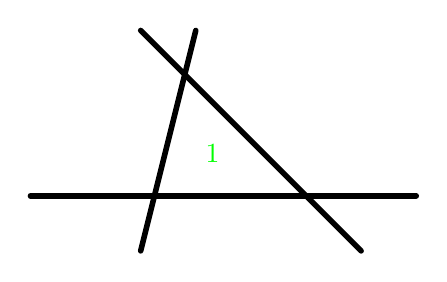
\begin{tikzpicture}[scale=0.7, line cap=round,line join=round,x=1.0cm,y=1.0cm]
	\draw [line width=2.pt] (0,-5)-- (1,-1);
	\draw [line width=2] (0,-1)-- (4,-5);
	\draw [line width=2] (-2,-4)-- (5,-4);
    \draw (1,-2.9) node[anchor=north west] {\color{green} $1$};
	\end{tikzpicture}
\end{center}
\end{minipage} 
\hfill
\begin{minipage}{0.49\linewidth} 
\begin{center}
	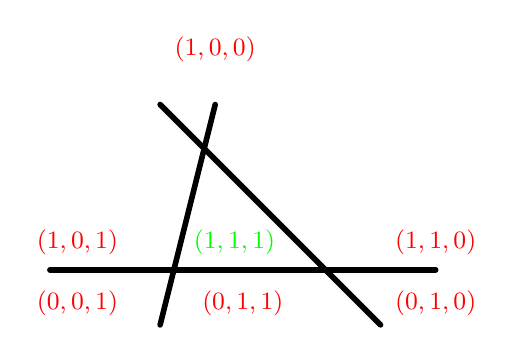
\begin{tikzpicture}[scale=0.7, line cap=round,line join=round,x=1.0cm,y=1.0cm]
	\draw [line width=2.pt] (0,-5)-- (1,-1);
	\draw [line width=2] (0,-1)-- (4,-5);
	\draw [line width=2] (-2,-4)-- (5,-4);
    \draw (1.35,-3.5) node {\small \color{green} $(1, 1, 1)$};
    \draw (-1.5,-3.5) node {\small \color{red} $(1, 0, 1)$};
    \draw (5,-3.5) node {\small \color{red} $(1, 1, 0)$};
    \draw (1.5,-4.6) node {\small \color{red} $(0, 1, 1)$};
    \draw (-1.5,-4.6) node {\small \color{red} $(0, 0, 1)$};
    \draw (5,-4.6) node {\small \color{red} $(0, 1, 0)$};
    \draw (1,0) node {\small \color{red} $(1, 0, 0)$};
	\end{tikzpicture}
\end{center}
\end{minipage} 

\item Первый слой должен построить нам три линии. Это три нейрона. Второй слой должен принять решение в какой из полос мы оказались. Будем считать, что если мы попали направо, нейрон выдаёт единицу. Если мы попали налево, ноль. В качестве функции активации используем единичную ступеньку. 

\begin{minipage}{0.49\linewidth} 
\begin{center}
	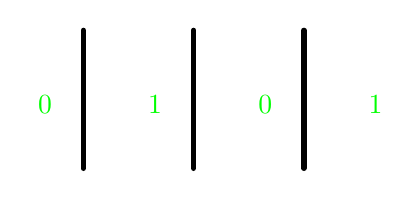
\begin{tikzpicture}[scale=0.7, line cap=round,line join=round,x=1.0cm,y=1.0cm]
	\draw [line width=2.pt] (0,-1.5)-- (0,1);
	\draw [line width=2.pt] (2,-1.5)-- (2,1);
	\draw [line width=2.pt] (4,-1.5)-- (4,1);
    \draw (-1,0) node[anchor=north west] {\color{green} $0$};
    \draw (1,0) node[anchor=north west] {\color{green} $1$};
    \draw (3,0) node[anchor=north west] {\color{green} $0$};
    \draw (5,0) node[anchor=north west] {\color{green} $1$};
	\end{tikzpicture}
\end{center}
\end{minipage} 
\hfill
\begin{minipage}{0.49\linewidth} 
\begin{center}
	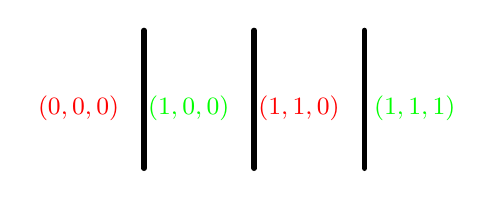
\begin{tikzpicture}[scale=0.7, line cap=round,line join=round,x=1.0cm,y=1.0cm]
	\draw [line width=2.pt] (0,-1.5)-- (0,1);
	\draw [line width=2.pt] (2,-1.5)-- (2,1);
	\draw [line width=2.pt] (4,-1.5)-- (4,1);
    \draw (-2.1,0) node[anchor=north west] {\small \color{red} $(0,0,0)$};
    \draw (-0.1,0) node[anchor=north west] {\small \color{green} $(1,0,0)$};
    \draw (1.9,0) node[anchor=north west] {\small \color{red} $(1,1,0)$};
    \draw (4,0) node[anchor=north west] {\small \color{green} $(1,1,1)$};
	\end{tikzpicture}
\end{center}
\end{minipage} 

Вопрос в том, хватит ли нам на втором слое одного нейрона для того, чтобы обработать все четыре возможные ситуации. Нам нужно, чтобы выполнялись следующие условия

\begin{equation*}
    \begin{cases} 
    & f(1 \cdot w_1 + 1 \cdot w_2 + 1 \cdot w_3) = 1 \\ 
    & f(1 \cdot w_1 + 0 \cdot w_2 + 0 \cdot w_3) = 0 \\
    & f(1 \cdot w_1 + 1 \cdot w_2 + 01 \cdot w_3) = 0 \\
    & f(0 \cdot w_1 + 0 \cdot w_2 + 0 \cdot w_3) = 0 \\
    \end{cases}.
\end{equation*}

Для того, чтобы со вторым уравнением всё было хорошо, возьмём $w_1 = 1.$ Тогда вес $w_2$ надо взять отрицательным, а $w_3$ положительным, например, $w_2 = -2$, а $w_3 = 4$. Тогда один нейрон на внешнем слое решит нашу задачу. Выходит, что всего надо задействовать 4 нейрона. 

\item Оценим число нейронов сверху. Перед нами две $XoR$ задачи, которые лежат рядом с друг-другом. Для решения каждой надо $3$ нейрона. Чтобы объединить получившиеся решения нужен ещё один нейрон. Получается трёхслойная сетка с $7$ нейронами.

Если мы попробуем подойти к задаче также, как в предыдущем пункте, на втором слое мы получим несовместимую систему из уравнений. То есть третьего слоя точно не избежать. 

Можно первым слоем построить $3$ линии, вторым решить задачу из предыдущего пункта, а на третьем добавить информацию о том, выше горизонтальной линии мы оказались или ниже. Тогда мы потратим $6$ нейронов. Нейросетка получится неполносвязной. 

\begin{center}
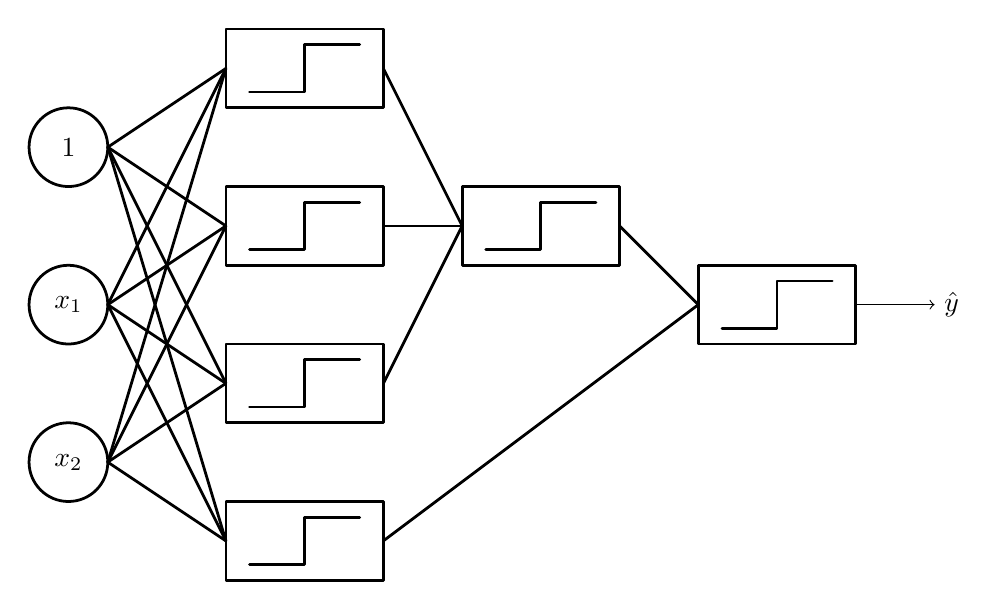
\begin{tikzpicture}[line cap=round,line join=round,x=1.0cm,y=1.0cm]

\draw [line width=1.pt] (-3,1.5) circle (0.5cm) node {$1$};
\draw [line width=1.pt] (-3,-0.5) circle (0.5cm) node {$x_1$};
\draw [line width=1.pt] (-3,-2.5) circle (0.5cm) node {$x_2$};	

\draw [line width=1.pt] (-1,2)--(1,2)--(1,3)--(-1,3)--cycle;
\draw [line width=1.pt] (-0.7,2.2)--(0,2.2)--(0,2.8)--(0.7,2.8);

\draw [line width=1.pt] (-1,0)--(1,0)--(1,1)--(-1,1)--cycle;
\draw [line width=1.pt] (-0.7,0.2)--(0,0.2)--(0,0.8)--(0.7,0.8);

\draw [line width=1.pt] (-1,-2)--(1,-2)--(1,-1)--(-1,-1)--cycle;
\draw [line width=1.pt] (-0.7,-1.8)--(0,-1.8)--(0,-1.2)--(0.7,-1.2);

\draw [line width=1.pt] (-1,-3)--(1,-3)--(1,-4)--(-1,-4)--cycle;
\draw [line width=1.pt] (-0.7,-3.8)--(0,-3.8)--(0,-3.2)--(0.7,-3.2);

\draw [line width=1.pt] (-2.5,1.5) -- (-1,0.5);
\draw [line width=1.pt] (-2.5,1.5) -- (-1,2.5);
\draw [line width=1.pt] (-2.5,1.5) -- (-1,-1.5);
\draw [line width=1.pt] (-2.5,1.5) -- (-1,-3.5);

\draw [line width=1.pt] (-2.5,-0.5) -- (-1,0.5);
\draw [line width=1.pt] (-2.5,-0.5) -- (-1,2.5);
\draw [line width=1.pt] (-2.5,-0.5) -- (-1,-1.5);
\draw [line width=1.pt] (-2.5,-0.5) -- (-1,-3.5);

\draw [line width=1.pt] (-2.5,-2.5) -- (-1,0.5);
\draw [line width=1.pt] (-2.5,-2.5) -- (-1,2.5);
\draw [line width=1.pt] (-2.5,-2.5) -- (-1,-1.5);
\draw [line width=1.pt] (-2.5,-2.5) -- (-1,-3.5);

\draw [line width=1.pt] (2,0)--(4,0)--(4,1)--(2,1)--cycle;
\draw [line width=1.pt] (2.3,0.2)--(3,0.2)--(3,0.8)--(3.7,0.8);

\draw [line width=1.pt] (1,0.5) -- (2, 0.5);
\draw [line width=1.pt] (1,2.5) -- (2, 0.5);
\draw [line width=1.pt] (1,-1.5) -- (2, 0.5);

\draw [line width=1.pt] (5,0)--(7,0)--(7,-1)--(5,-1)--cycle;
\draw [line width=1.pt] (5.3,-0.8)--(6,-0.8)--(6,-0.2)--(6.7,-0.2);

\draw [line width=1.pt] (4,0.5) -- (5, -0.5);
\draw [line width=1.pt] (1,-3.5) -- (5, -0.5);

\draw [->] (7,-0.5) -- (8,-0.5) node[right] {$\hat y$};
\end{tikzpicture}
\end{center}

\item Думайте, рассуждайте, а автор умывает руки.
\end{enumerate} 
\end{sol} 


%%%-------------------------------------------
\begin{problem}{(универсальный регрессор)}
Маша доказала Паше, что у неё всё в полном порядке с логикой. Теперь она собирается доказать ему, что с помощью двухслойной нейронной сетки можно приблизить любую непрерывную функцию от одного аргумента $f(x)$ со сколь угодно большой точностью\footnote{\url{http://neuralnetworksanddeeplearning.com/chap4.html}}.  

\textbf{Hint:}  Вспомните, что любую непрерывную функцию можно приблизить с помощью кусочно-линейной функции (ступеньки). Осознайте как с помощью пары нейронов можно описать такую ступеньку. Соедините все ступеньки в сумму с помощью выходного нейрона. 
\end{problem}

\begin{sol}
% https://medium.com/analytics-vidhya/you-dont-understand-neural-networks-until-you-understand-the-universal-approximation-theorem-85b3e7677126

Не нужно воспринимать эту задачку как строгое доказательство. Скорее, это показательство. Мы хотим приблизить функцию $f(x)$ с какой-то точностью. Будем делать это с помощью кусочно-линейных ступенек. Чем выше точность, тем больше будем рисовать ступенек.

\begin{center}
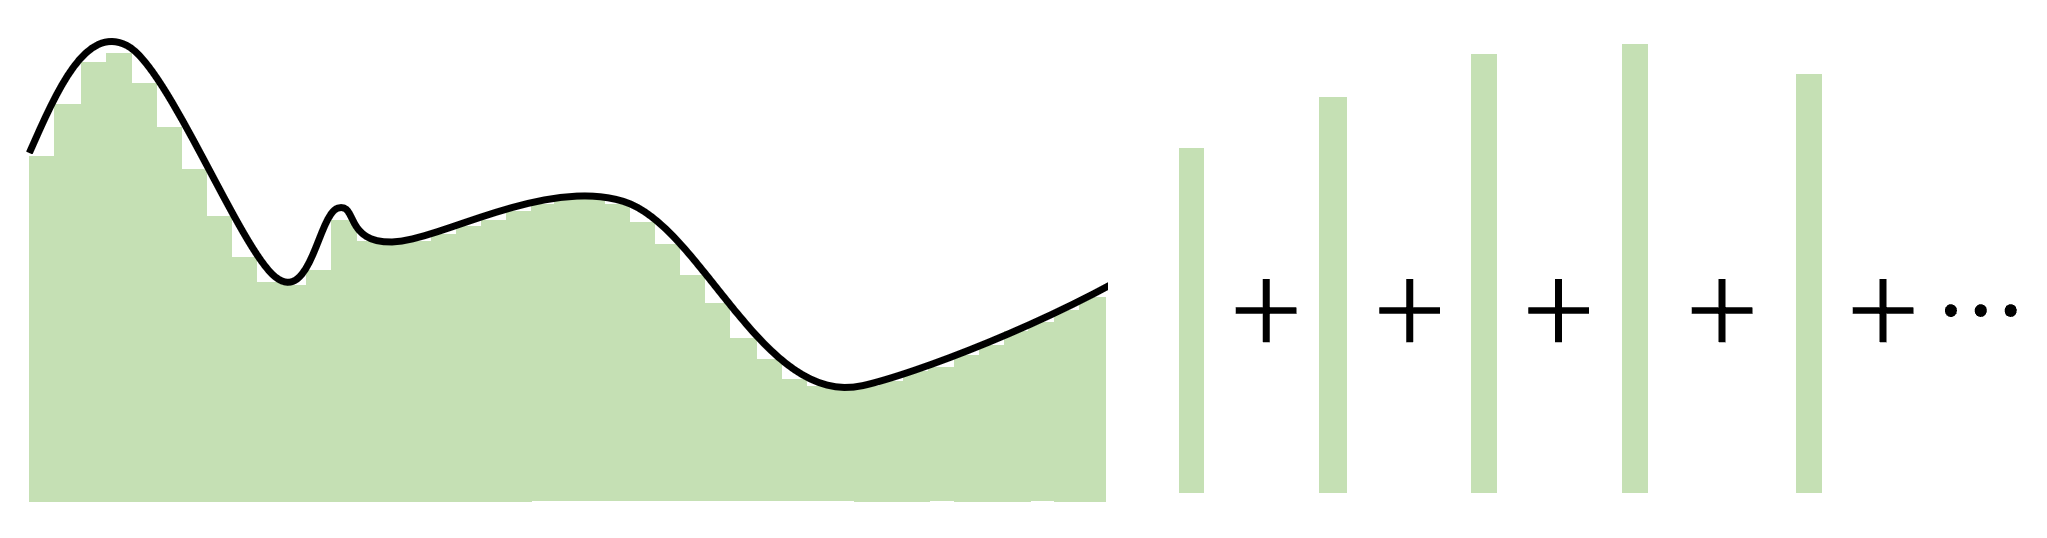
\includegraphics[scale=0.2]{images/steps.png}
\end{center}

Высоту ступеньки определяют по-разному. Чаще всего как значение функции в середине выбранного отрезка $b_i = f(\frac{a_i + a_{i+1}}{2})$. Тогда всю функцию целиком можно приблизить суммой

$$
f(x) \approx \sum_{i=1}^n f \left( \frac{a_i + a_{i+1}}{2} \right) \cdot [a_i \ge x < a_{i+1}].
$$

Давайте попробуем описать с помощью нейрона одну из ступенек. Пуст высота этой ступеньки равна $b_i$. Шагать по оси $x$ мы будем с фиксированным шагом $h$, поэтому $a_{i+1} = a_i + h$.

\begin{center}
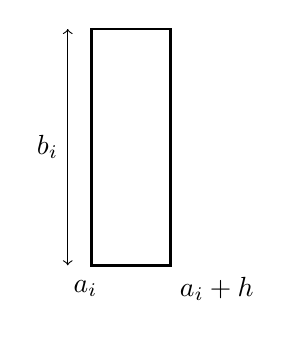
\begin{tikzpicture}
\draw [line width=1.pt] (0,0)--(1,0)--(1,3)--(0,3)--cycle;
\draw [->] (-0.3,0)--(-0.3,3);
\draw [->] (-0.3,3)--(-0.3,0);
\draw (-0.3, 1.5) node[left] {$b_i$};
\draw (0.2, -0.3) node[left] {$a_i$};
\draw (1, -0.3) node[right] {$a_i + h$};
\end{tikzpicture}
\end{center}

Если $x$, для которого мы ищем $f(x)$ попадает в полуинтервал, на котором задана наша ступенька, мы будем приближать $f(x)$ этой ступенькой. Ступенька состоит из двух линий. Выходит, что она будет описываться двумя нейронами. Если мы внутри ступеньки, значит $a_i \le x < a_i + h$. Пара нейронов должна сравнить $x$ с $a_i$ и $a_i + h$ и на основе этого принять решение. Можно записать попадание $x$ в ступеньку следующим образом:

$$
1 - [x < a_i] - [x \ge a_i + h]
$$

Если оба условия --- неправда, получаем $1$. Мы в ступеньке. Если хотя бы одно из них выполнено --- мы вылетаем за ступеньку. Оба сразу выполниться они не могут. Нарисуем это в виде нейрона. В качестве функции активации используем единичную ступеньку. 

\begin{center}
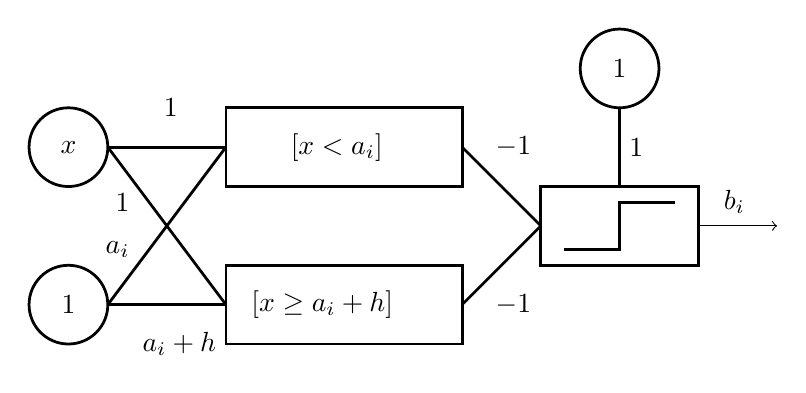
\begin{tikzpicture}
\draw [line width=1.pt] (-3, 1.5) circle (0.5cm) node {$x$};
\draw [line width=1.pt] (-3, -0.5) circle (0.5cm) node {$1$};
	
\draw [line width=1.pt] (-1,1)--(2,1)--(2,2)--(-1,2)--cycle;
\draw (-0.3, 1.5) node[right] {$[x < a_i]$};

\draw [line width=1.pt] (-1,-1)--(2,-1)--(2,0)--(-1,0)--cycle;
\draw (-0.8, -0.5) node[right] {$[x \ge a_i + h]$};

\draw [line width=1.pt] (-2.5,1.5) -- (-1,1.5);
\draw (-1.7, 2) node {$1$};
\draw [line width=1.pt] (-2.5,1.5) -- (-1,-0.5);
\draw (-2.1, 0.8) node[left] {$1$};
\draw [line width=1.pt] (-2.5,-0.5) -- (-1,1.5);
\draw (-1, -1) node[left] {$a_i + h$};
\draw [line width=1.pt] (-2.5,-0.5) -- (-1,-0.5);
\draw (-2.1, 0.2) node[left] {$a_i$};

\draw [line width=1.pt] (3,0)--(5,0)--(5,1)--(3,1)--cycle;
\draw [line width=1.pt] (3.3,0.2)--(4,0.2)--(4,0.8)--(4.7,0.8);
\draw [line width=1.pt] (2,1.5) -- (3,0.5);
\draw (3, 1.5) node[left] {$-1$};
\draw [line width=1.pt] (2,-0.5) -- (3,0.5);
\draw (3, -0.5) node[left] {$-1$};

\draw [line width=1.pt] (4, 2.5) circle (0.5cm) node {$1$};
\draw [line width=1.pt] (4,2) -- (4,1);
\draw (4, 1.5) node[right] {$1$};

\draw [->] (5,0.5) -- (6,0.5);
\draw (5.2, 0.8)  node[right] {$b_i$};
\end{tikzpicture}
\end{center}

Нарисуем такую сетку для каждой ступеньки. Если мы попали в ступеньку, сетка будет выплёвывать со второго слоя единичку. Там мы будем умножать её на $b_i$ и посылать на внешний слой. Мы всегда будем попадать только в одну из ступенек, значит только один из слоёв выдаст нам $1$. Все остальные выдадут $0$. На внешнем слое нам остаётся только просуммировать всё, что к нам пришло и выдать ответ. Чем больше ступенек мы добавляем в модель, тем точнее наша апроксимация. 
\end{sol} 

% \newpage 

%%%-------------------------------------------
\begin{problem}{(число параметров)}
Та, кому принадлежит машин лёрнинг собирается обучить полносвязную нейронную сеть для решения задачи регрессии, На вход в ней идёт $12$ переменных, в сетке есть $3$ скрытых слоя. В первом слое $300$ нейронов, во втором $200$, в третьем $100$.  Сколько параметров предстоит оценить Маше?
\end{problem}

\begin{sol} 
Нам нужно решить довольно простую комбинаторную задачку. Связи в нашей сетке проведены между всему нейронами. Не забываем учесть, что у каждого нейрона есть константа. Получается, что всего параметров будет

\[
(12 + 1) \cdot 300 + (300 + 1) \cdot 200 + (200 + 1) \cdot 100 + (100 + 1) \cdot 1.
\]

\end{sol} 
